\chapter{Population modelling}

When modelling the changes to any population we must ensure that we include any pertinent production sources and removal sinks. This ensures that we maintain ``population conservation''. Namely, all creation and degradation  is accounted for in the following word equation \see{Conservation},
\bb
\textrm{Rate of population change}= \textrm{Birth
Rate} - \textrm{Death Rate}   + \textrm{Rate of
Immigration} - \textrm{Rate of Emigration}\nonumber
\ee
\begin{figure}[!!!h!!!tb]
\centering
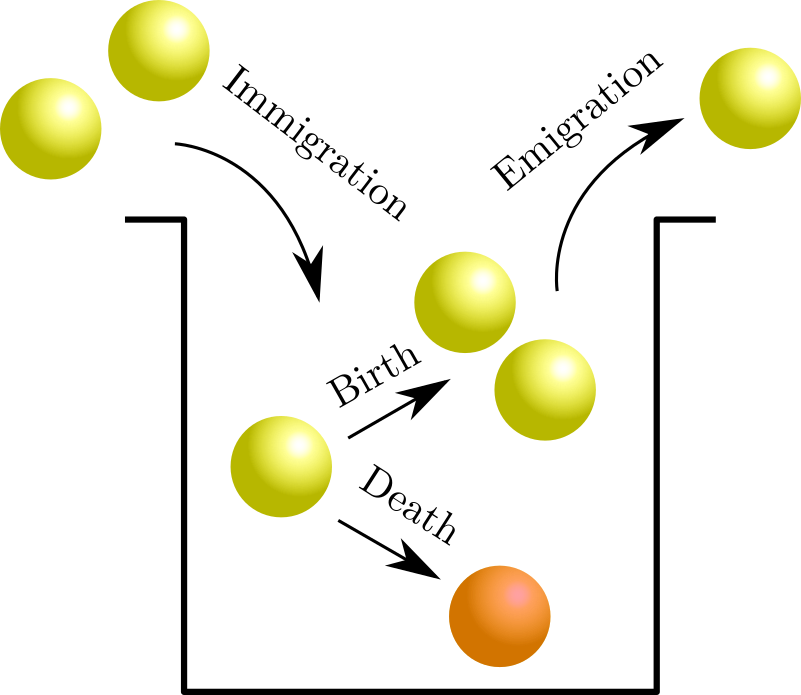
\includegraphics[width=\ttp]{../Pictures/Conservation.png}
\caption{\label{Conservation}Population changes stem from four basic dynamics.}
\end{figure}

In this chapter we assume that the system is closed and thus there is no emigration of immigration. Namely, we assume that the problem has no spatial variation, or that it is not important. Thus we simply consider the temporal evolution of the system.

\section{Continuum modelling}
There are multiple ways of modelling a population. If there are a large number of individuals in the population and we want to consider how the population changes over continuous time we can use ODEs to define the rules governing the evolution and, hence, predict how the population will fair.
\begin{defin}
Suppose there exists a function $g$ such that $\dot{u}=f(u)$ can be written as 
\bb
\dot{u}=ug(u)
\ee
then $g$ is known as the intrinsic growth rate.
\end{defin}

\begin{example}[frametitle=Growth law examples]\label{Growth examples}

\begin{itemize}
\item The Malthus model, 1798
\begin{align}
u&\stackrel{b}{\rightarrow}2u,\nonumber\\
u&\stackrel{d}{\rightarrow}\slashed{0}.\nonumber
\end{align}
\COL{From the law of mass action we get
\bb
\dot{u}=u(b-d)\quad u(0)=u_0.\label{Malthus_model}
\ee
Equation \eqref{Malthus_model} can easily be solved to produce the solution $u=u_0\exp\l (b-d)t \r$. However, we can get all the information from \eqn{Malthus_model} just from considering different cases of $b$ and $d$. Namely,
\bb
u\textrm{ is }\left\{
\begin{array}{rl}
      \textrm{exponentially growing if} & b>d, \\
\textrm{not changing if} & b=d, \\
      \textrm{exponentially decaying if} & b<d.
\end{array} \right.
\ee
}

\item The Verhulst Model, 1845. Also commonly known as the Logistic Growth Model.
\begin{align}
u&\stackrel{r}{\rightarrow}2u,\nonumber\\
2u&\stackrel{r/K}{\rightarrow}u.\nonumber
\end{align}
\COL{The Logistic equation is
\bb
\dot{u}=ru\l 1-\frac{u}{K}\r\nonumber
\ee
Using partial fractions, we can directly solve for $u$. Specifically,
\begin{align}
\frac{\rd u}{\rd t}&=ru\l 1-\frac{u}{K}\r,\nonumber\\
\Rightarrow\int_0^T\frac{\rd u}{u(1-u/K)}&=\int_0^Tr \rd t,\nonumber\\
\Rightarrow\int_0^T \frac{1}{u}+\frac{1/K}{1-u/K}  \rd u&=rT,\nonumber\\
\Rightarrow\left[\ln(u)-\ln\l 1- \frac{u}{K} \r \right]^T_0&=rT,\nonumber\\
\Rightarrow\ln\l\frac{u}{1- \frac{u}{K}} \r-\ln\l\frac{u_0}{1- \frac{u_0}{K}} \r&=rT,\nonumber\\
\Rightarrow u(T)&=\frac{K}{1+\frac{K-u_0}{u_0}\exp\l{-rT}\r}.
\end{align}
}
\end{itemize}
\end{example}

\begin{example}[frametitle=US population]\label{US population}
In 1845 Pierre Verhulst used 60 years worth of population data from the US census and was able to predict the population for the next 100 years. See Table \ref{US_census_data} and \fig{US_population_prediction}.
\begin{itemize}
\item What goes wrong after 1950 in \fig{US_population}?
\item In \fig{US_population_2030} one of the fitted parameters is $K=309.3$. What does this mean?
\item The US population in 2018 was over 327 million. Should we use the logistic equation to model the US population? 
\end{itemize}

 \COL{
\begin{itemize}
\item Multiple possible answers: the second world war created the baby boomer generation, who produced a lot of children; medicine/ hygiene/ food production became a lot better after the second world war due to scientific advances and operations research.
\item It suggests that the maximum population of the US should be around 309 million. 
\item Could be answered both yes or no. 
\begin{itemize}
\item Yes: there is certainly going to be a fundamental limit the US can sustain (the carrying capacity). The current population is within $\pm10\%$ of the prediction, so not too bad.
\item No: we do not know what the limiting factors are so, we cannot encode them in the equation. The logistic equation contains an exponential factor, meaning that the results are very sensitive to small changes. The model assumes the population does not have external interference and, so, diseases, wars, and/or technological advances, which can fundamentally change a population are not considered.
\end{itemize}
\end{itemize}}
\end{example}

\begin{table}[!!!h!!!tbp]
\resizebox{\textwidth}{!}{%
\begin{tabular}{ccc}
\hline
\textbf{Year} & \textbf{US census data in millions} & \textbf{Population prediction in millions} \\ \hline\hline
\textbf{1790} & \textbf{3.929}  & \textbf{3.929}  \\ \hline
\textbf{1800} & \textbf{5.308}  & \textbf{5.346}  \\ \hline
\textbf{1810} & \textbf{7.240}  & \textbf{7.255}  \\ \hline
\textbf{1820} & \textbf{9.638}  & \textbf{9.808}  \\ \hline
\textbf{1830} & \textbf{12.866} & \textbf{13.195} \\ \hline
\textbf{1840} & \textbf{17.069} & \textbf{17.635} \\ \hline
1850          & 23.192          & 23.3700          \\ \hline
1860          & 31.443          & 30.635         \\ \hline
1870          & 38.558          & 39.616          \\ \hline
1880          & 50.156          & 50.388         \\ \hline
1890          & 62.948          & 62.851         \\ \hline
1900          & 75.996          & 76.681          \\ \hline
1910          & 91.972          & 91.339         \\ \hline
1920          & 105.711         & 106.132        \\ \hline
1930          & 122.775         & 120.346        \\ \hline
1940          & 131.669         & 133.373         \\ \hline
1950          & 150.697         & 144.802         \\ \hline
1960          & 179.323         & 154.455         \\ \hline
1970          & 203.185         & 162.347        \\ \hline
1980          & 226.546         & 168.630         \\ \hline
1990          & 248.710         & 173.527         \\ \hline
\end{tabular}%
}
\caption{\href{https://www.census-charts.com/Population/pop-us-1790-2000.html}{US population census data} between 1790 and 1990 and the accompanying prediction by the logistic equation. The bold data at the top was all that was known to Verhulst in 1845.\label{US_census_data}}
\end{table}
\begin{figure}[!!!h!!!tb]
\centering
\subfigure[\label{US_population}]{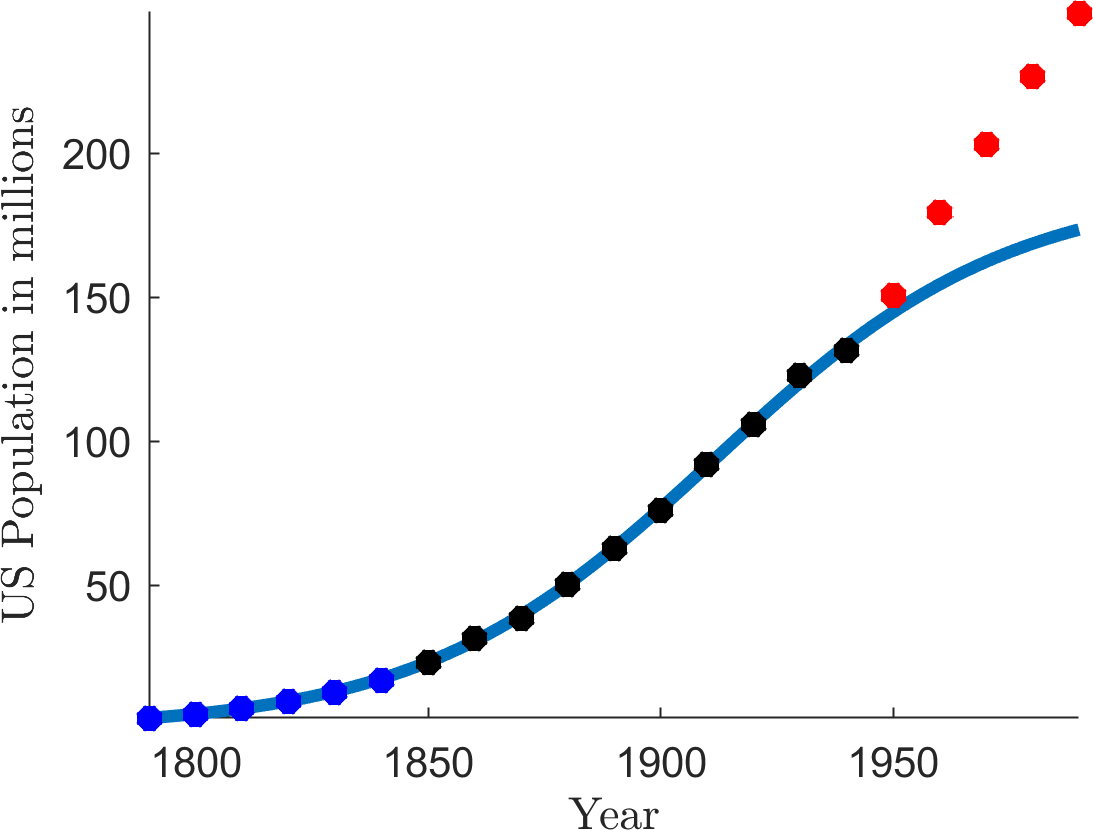
\includegraphics[width=\ttp]{../Pictures/US_logistic_population.png}}
\subfigure[\label{US_population_2030}]{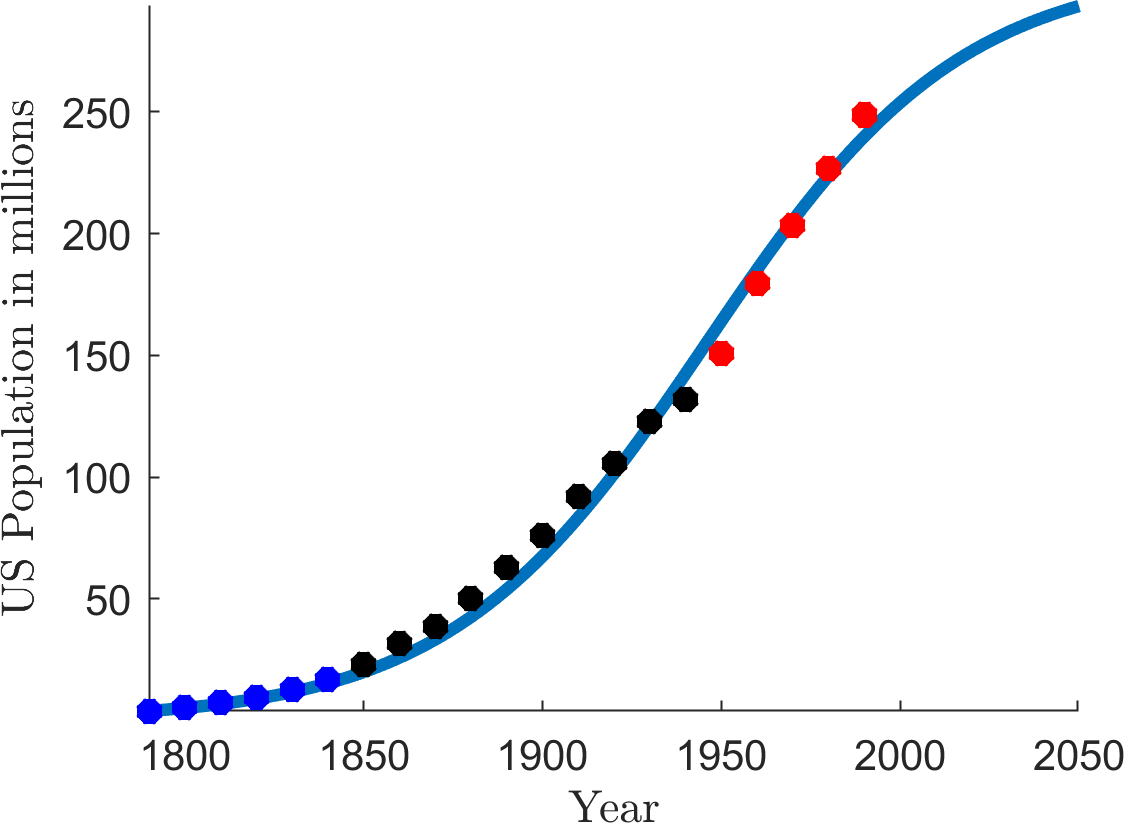
\includegraphics[width=\ttp]{../Pictures/US_logistic_population_2030.png}}
\caption{(a) The logistic curve fitted by Verhulst in 1845 to US census data. The blue dots are the data known to Verhulst. The black data is the next 100 years worth of data.  The initial condition is given by the data $u_0=3.929$. The fitted parameters are $K=188.3$ and $r=0.0316$. (b) The logistic curve fitted with all data up to 1990. The fitted parameters are $K=309.3$ and $r=0.0280$. See example \ref{US population}. \label{US_population_prediction}}
\end{figure}

\newpage
\begin{figure}[h!!!tb]
\centering
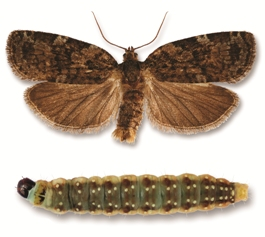
\includegraphics[width=\ttp]{../Pictures/Spruce_budworm.jpg}
\caption{\label{Spruce_budworm} Spruce budworm in moth and larval stages.}
\end{figure}
\begin{example}[frametitle=Spruce budworm]\label{Spruce budworm}
Spruce budworm \see{Spruce_budworm} are preyed upon by spiders, miscellaneous insects, and birds. A model for their population size, $N$ is given by
\bb
\dot{N}=RN\l 1-\frac{N}{K}\r-\frac{BN^2}{A^2+N^2}.\label{Spruce_eqn}
\ee
\begin{enumerate}
\item What does each term in the equation mean?
\item Describe, with a sketch, three properties of the predation term
\bb
\frac{BN^2}{A^2+N^2}.
\ee
Hint: consider low, medium and high values of $N$.
\item Non-dimensionalise the equation to give the form
\bb
\frac{\rd u}{\rd \tau}=\underbrace{ru\l 1-\frac{u}{k}\r}_{f_1(u)}-\underbrace{\frac{u^2}{1+u^2}}_{f_2(u)}.
\ee
\item By sketching the two terms, $f_1$ and $f_2$ separately, show there are between 2 and 4 steady states (depending on the values of $(r,k)$).
\item By considering the $f_1-f_2$ sketches, characterise the steady state stabilities in all cases.
\item Spruce budworm destroys spruce trees and, so, we would like there population to be extinct. However, what can happen if there is a large outbreak?
\end{enumerate}


\begin{enumerate}
\item \COL{
\bb
\underbrace{\dot{N}}_{\textrm{Population evolution.}}=\underbrace{RN\l 1-\frac{N}{K}\r}_{\textrm{Logistic growth, \ie linear growth with competition.}}-\underbrace{\frac{BN^2}{A^2+N^2}}_{\textrm{Predation effects.}}.
\ee}



\item \COL{For low populations there is little predation. As the population grows, so does the predation. The predation saturates at large population.}


\item \COL{We have two degrees of freedom, $N=[N]u$ and $t=[t]\tau$, so we need two balances. Comparing the original equation with the equation we want we see that the balances are}
\bb
\tikzmark{a}\dot{N}=RN\l 1-\frac{N}{K}\r-\tikzmark{b}BN^2/\l \tikzmark{c}A^2+\tikzmark{d}N^2\r,
\tikz[overlay,remember picture]
{\draw[square arrow1] (a.south east) to (b.south east);}
\tikz[overlay,remember picture]
{\draw[square arrow2] (c.south east) to (d.south east);}
\ee
\COL{which give the follows equalities:
\bb
\frac{[N]}{[t]}=B, \quad [N]^2=[A]^2.
\ee
Hence,
\bb
[N]=A,\quad [t]=\frac{A}{B}.
\ee
Note that you have to be careful because the dimensions of the $N^2$ in the numerator of the predation fraction cancel with those in the denominator.

Substituting these into \eqn{Spruce_eqn} we get
\bb
B\dot{u}=R[N]u\l 1-\frac{[N]u}{K}\r-\frac{B[N]}{A}\frac{u^2}{1+u^2}.\nonumber
\ee
Divide through by $B$ and replace $[N]$ with $A$ to get
\bb
\dot{u}=\frac{RA}{B}u\l 1-\frac{Au}{K}\r-\frac{u^2}{1+u^2}.\nonumber
\ee
Finally, we can see that
\bb
r=\frac{RA}{B},\quad k=\frac{K}{A}.
\ee}



\item \COL{See \fig{Spruce_budworm_phase_plane}. We approach the sketching via the following steps:}
\begin{itemize}


\item \COL{Note any ``obvious'' crossings, \ie $u=0,1,$ or immediate parameter dependencies. Here, we see that both terms cross at $0$, thus, there is at least one steady state.}


\item \COL{Next, consider the derivatives at these obvious points. Namely, $u^2/(1+u^2)$ has $0$ derivative at $u=0$, whereas $ru(1-u/k)$ has derivative $r>0$ at $u=0$. Thus, at least for a small interval of $u$ near zero, $f_2>f_1$}


\item \COL{Consider the dynamics for large values of $u$. Here, $f_1\rightarrow 1$, whilst $f_2\rightarrow -\infty$. }


\item \COL{Combining the two previous points that initially $f_2>f_1$ but eventually $f_2<f_1$ means that there must be at least one more crossing for $u>0$ (see left and right of \fig{Spruce_budworm_phase_plane} in particular).}


\item \COL{Consider what each parameter does. Namely, $k$ controls the width of the logistic parabola of $f_1$, whereas $r$ controls the height. Playing around with multiple sketches, we will eventually find the middle case of \fig{Spruce_budworm_phase_plane}.}
\end{itemize}

\item \COL{By considering the bottom row of figures we can characterise the stability of the steady states. Firstly, $u_c=0$ is always unstable. Whenever there two steady states $u_{c1}=0$ and the larger state $u_{c2}>u_{c1}$ the larger steady state is always stable. Whenever there are four steady states we denote them $u_{c1}<u_{c2}<u_{c3}<u_{c4}$ and note that $u_{c1}$ and $u_{c3}$ are unstable, whilst $u_{c2}$ and $u_{c4}$ are stable.}
\item \COL{Unfortunately, the extinction state is never stable. Thus, trying to destroy them all is futile because if any are left the will repopulate their species. In the case of a big outbreak, $r>>1$, which means that the population will evolve to the large population state. Even if the growth rate, $r$, is returned to normal the population will remain at the larger population. Thus, this system exhibits hysteresis, and $r$ would have to be reduced beyond its original value, before the population would collapse back to its original population.}
\end{enumerate}
\end{example}

\begin{figure}[h!!!tb]
\centering
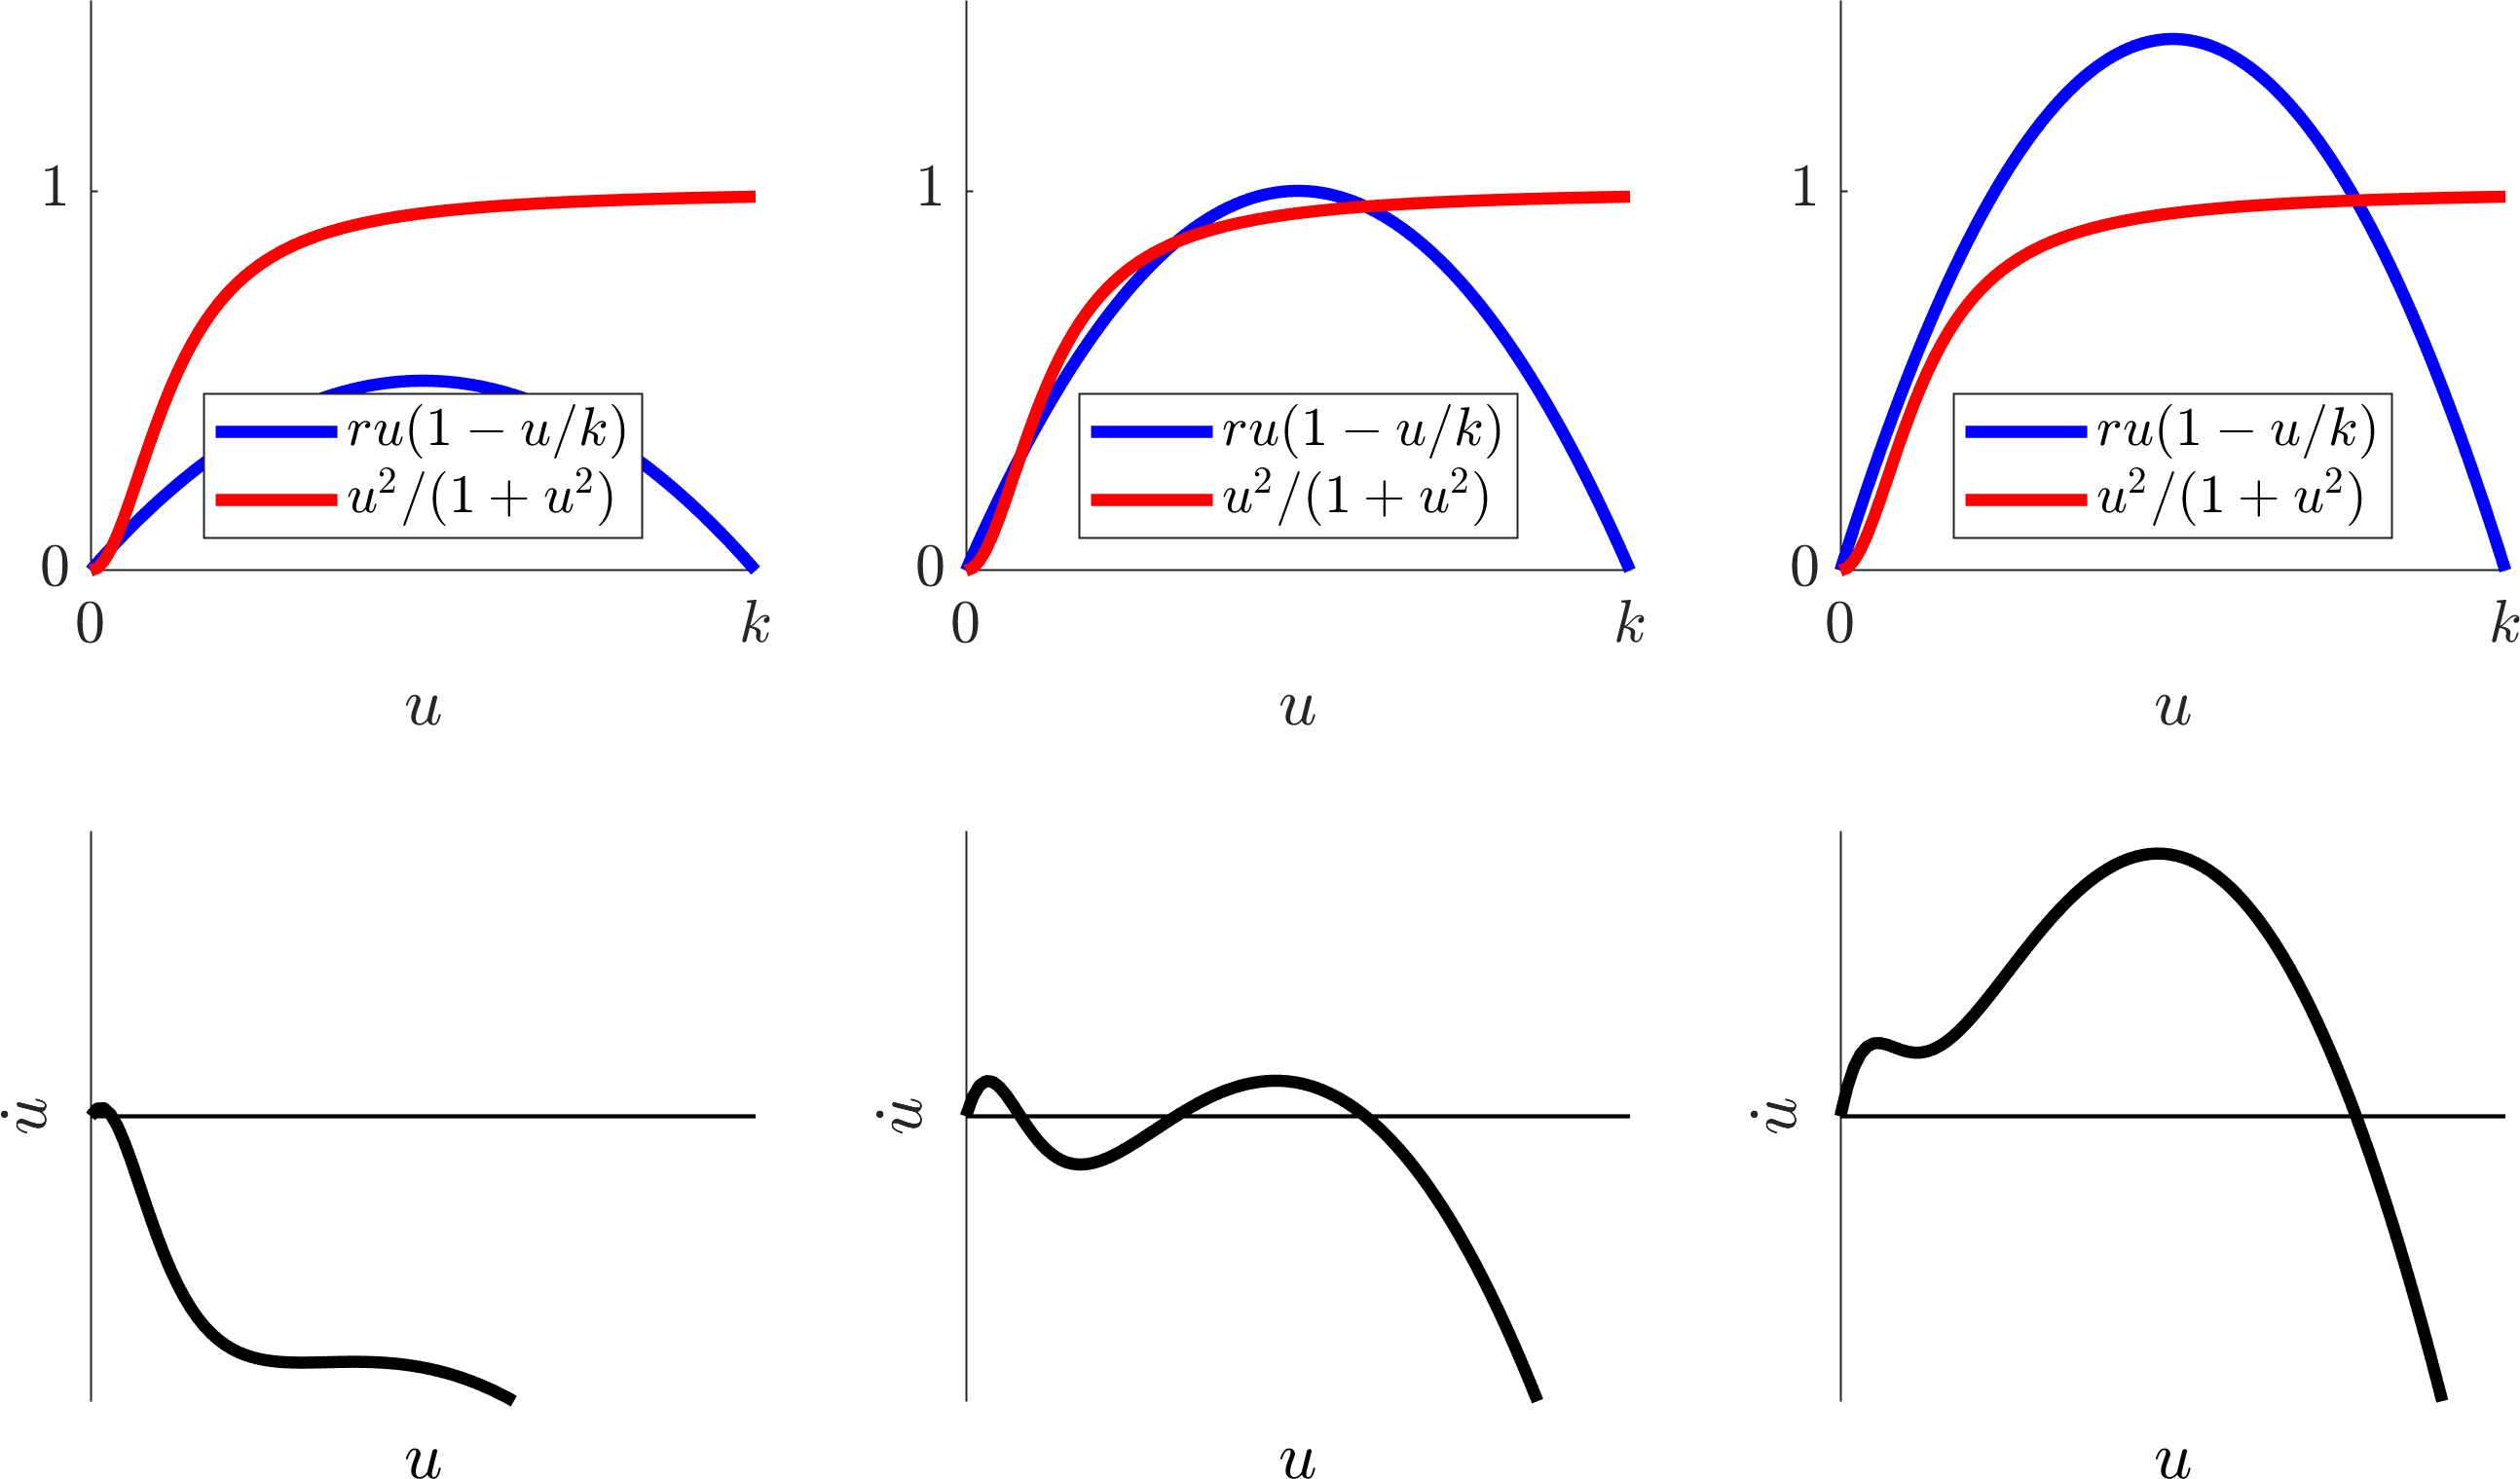
\includegraphics[width=\tp]{../Pictures/Spruce_budworm_phase_plane.png}
\caption{\label{Spruce_budworm_phase_plane} Parameter dependence of the Spruce budworm dynamics. $r$ is increasing left to right. The top images are plots of $f_1$ and $f_2$, whilst the bottom illustrates the phase plane $(u,\dot{u}=f_1-f_2)$.}
\end{figure}




\subsection{Disease transmission}

The study of infectious diseases has a long history and there are numerous, detailed models of a variety of epidemics and epizootics (i.e. animal epidemics). We can only possibly scratch the surface. In the following, we  consider a simple, framework, model but even this is  capable of highlighting general comments about epidemics and, in fact, approximately describe some specific epidemics.

Critically, one of the questions we will seek to answer is when is does a disease become an epidemic? Once we have set up the mathematical description of the disease we will see that converting the idea of an epidemic as an increasing number of infections will be fairly simple.


We consider a disease for which the population can be placed into 3 compartments:
\begin{itemize}
\item a Susceptible compartment, $S$, who can catch the disease.
\item an Infective compartment, $I$, who have and transmit the disease.
\item a Removed compartment, $R$, who have been isolated, or who have
recovered and are immune to the disease, or have died due to the
disease during the course of the epidemic.
\end{itemize}
In order to derive the equations we make the following assumptions:
\begin{itemize}
\item The disease is of short duration course so that the population is constant (counting those who have died due to the disease during the course of the epidemic).
\item The disease has a negligible incubation period.
\item If a person contracts the disease and recovers, they are immune (and hence remain in the removed compartment).
\item The numbers involved are sufficiently large to justify a continuum approximation.
\end{itemize}

\begin{figure}[h!!!tb]
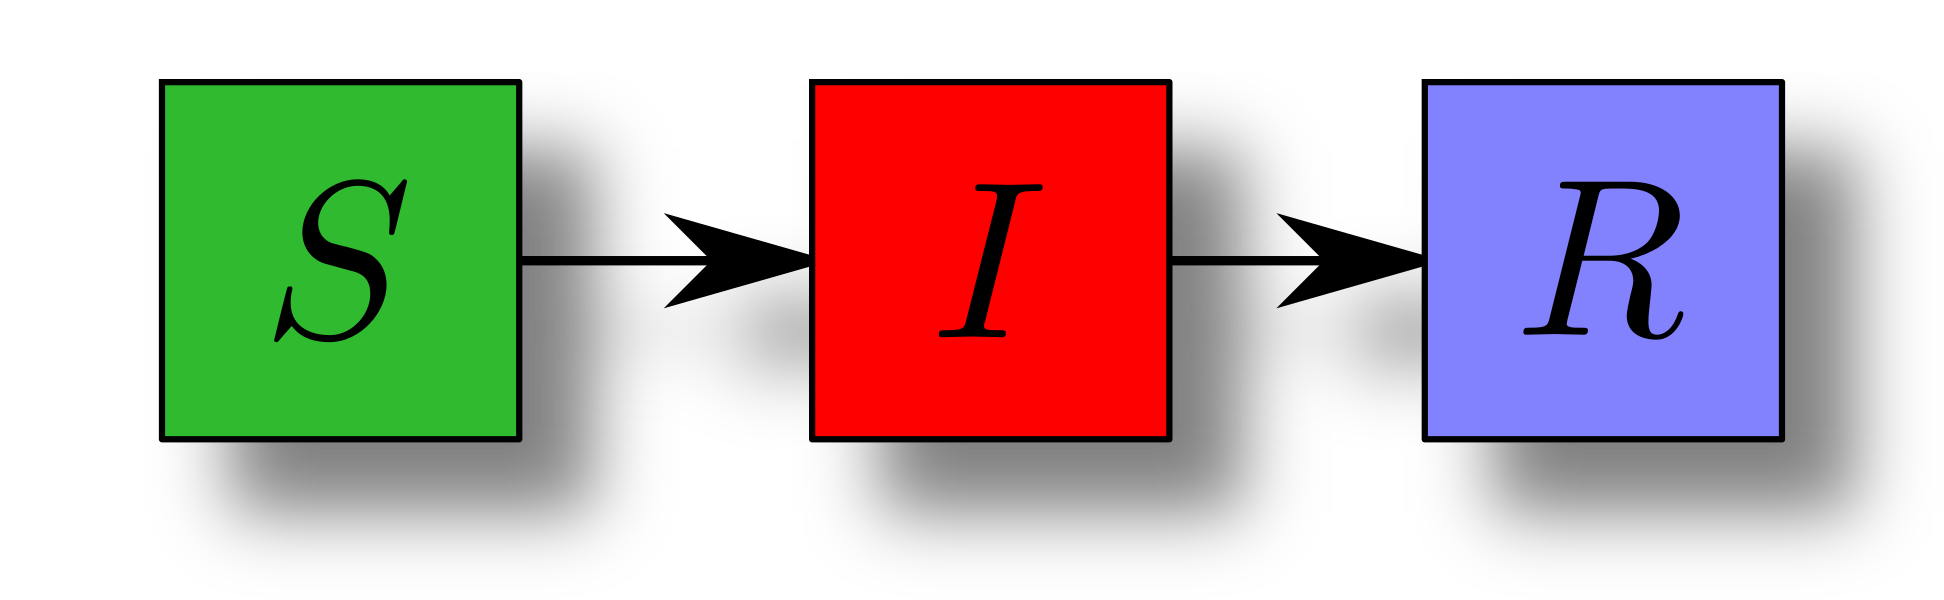
\includegraphics[width=\textwidth]{../Pictures/SIR.png}
\caption{Schematic view of a disease transmission. Susceptibles become infectious and, eventually, become removed from the system.}
\end{figure}

The `dynamics' of the disease can be described by applying a Law of Mass Action to
\begin{align}
S+I&\stackrel{r}{\rightarrow}2I,\\
I&\stackrel{a}{\rightarrow}R,
\end{align}
which provide the following ODEs:
\COL{
\begin{align}
\dot{S}&=-rSI,\label{S}\\
\dot{I}&=rSI-aI,\label{I}\\
\dot{R}&=aI.\label{R}
\end{align}
In terms of initial conditions we usually assume that there is no natural immunity, thus, $R_0=0$ because no one has yet recovered, died, or otherwise been removed from the disease. The other initial conditions, $(S_0,I_0)$, are unknown and can be treated as a parameters, or fitted to data.}

\begin{defin}
A disease is classed as an epidemic if the number of infections is growing in the population. Explicitly, an epidemic is occuring if $\dot{I}>0$.
\end{defin}

\begin{example}[frametitle=SIR questions \label{SIR}]
Suppose we know the parameters $r$ and $a$, which can be estimated from data then we develop methods to approach the following key questions.
\begin{enumerate}
\item Noting that $R$ decouples, construct a $(S,I)$ phase plane with nullclines and dynamic arrows to better understand the possible dynamics.

\COL{See \fig{SIR_phase_plane_trajectories}.}

\item Will the disease spread, \ie will the number of infectives increase, at least in the short-term?

\COL{
This question is asking if the number of infectives will increase initially. The number of infectives increases initially if and only if the derivative at time $t=0$ is positive, $rS_0I_0-aI_0>0$. Since $I_0>0$ we can simplify this comment to the number of infectives increases initially if and only if
\bb
\frac{rS_0}{a}>1.
\ee }
\begin{defin}
\bb
\rho=\frac{S_0r}{a}
\ee
is called the reproduction number. We can interpret $\rho$ as the average number of secondary infections that would be produced by one infective in a wholly susceptible population of size
$S_0$.
\end{defin}
Critically, we see here that an outbreak happens when $\rho>1$, whilst the infection dies out when $\rho<1$.

\item What will be the maximum number of infectives at any given time?


\begin{enumerate}
\item \COL{Notice that $\dot{R}$ can be decoupled from the system since \eqns{S}{I} are independent of $R$.}
\item \COL{From question 1 if $\rho<1$ then the number of infectives is decreasing, thus, in this case, the maximum number is the initial number $I_0$.}
\item \COL{If  $\rho>1$ then we have to do a bit more work. Namely, we have to evaluate $I_{\textrm{max}}$, critically, we note that at $I=I_{\textrm{max}}$ we must have $\dot{I}=0$ meaning that at the maximum point we have $S=a/r$. \label{crit_point}}
\item \COL{Notice that dividing \eqn{I} by \eqn{S} gives
\bb
\frac{\rd I/\rd t}{\rd S/\rd t}=\frac{\rd I}{\rd S}=-1+\frac{a}{rS},
\ee 
which can be integrated directly to
\bb
\int^I_{I_0}\rd I'=\int^S_{S_0}-1+\frac{a}{rS'}\rd S',
\ee
\bb
\implies I(t)-I_0=-S(t)+S_0+\frac{a}{r}\ln\l\frac{S(t)}{S_0}\r.\label{Infectives}
\ee
}
\item \COL{By point \ref{crit_point} we substitute $S=a/r$ into \eqn{Infectives}. Thus,
\bb
I_{\textrm{max}}=I_0+\frac{a}{r}-S_0+\frac{a}{r}\ln\l\frac{a}{rS_0}\r.
\ee
\item In summary
\bb
I_{\textrm{max}}=
\left\{
\begin{array}{ll}
      I_0 & \textrm{if } \rho<1, \\
      I_0+S_0-\frac{a}{r}+\frac{a}{r}\ln\l\frac{a}{rS_0}\r & \textrm{if }  \rho>1.
\end{array} 
\right.
\ee}
\end{enumerate}

\item How many people in total catch the disease?


\begin{enumerate}
\item \COL{Note that all infectives become removed eventually, thus, the total number that catch the disease is the total number of people in the removed category at the end of the infection, \ie far into the future. Call this number $R_\infty$.}


\item \COL{As time increases the number of infectives must eventually reduce because we have a finite population and at most everyone can have the infection once. Thus, $\lim_{t\rightarrow\infty} I(t)=0$.}


\item \COL{Using \eqn{Infectives}
\bb
\lim_{t\rightarrow\infty} I(t)=0=I_0-S_\infty+S_0+\frac{a}{r}\ln\l\frac{S_\infty}{S_0}\r.
\ee}



\item \COL{From adding \eqnto{S}{R} we see that $S+I+R=$ constant $=N=$ total population. Taking time to the two different limits of zero and infinity we can relate the initial condition and final steady states through $N$, namely,
\bb
N=S_0+I_0=S_\infty+R_\infty.
\ee
Hence,
\bb
R_\infty=N-S_\infty,
\ee
where $S_\infty$ satisfies the following equation
\bb
0=N-S_\infty+\frac{a}{r}\ln\l\frac{S_\infty}{S_0}\r.\label{S_Root}
\ee
Having derived \eqn{S_Root}, we must question the existence and uniqueness of potential solutions.

To check that at least one root exists we first rearrange \eqn{S_Root}
\bb
S_\infty-\frac{a}{r}\ln\l S_\infty\r=N-\frac{a}{r}\ln\l S_0\r\label{S_Root_rearranged},
\ee
where the right-hand side of \eqn{S_Root_rearranged} is just a constant. Thus, we have to sketch the left-hand side of \eqn{S_Root_rearranged} to get an idea of what the solution looks like.}



\item \COL{From \fig{Infection_schematic} we see that \eqn{S_Root} can have 0 to 2 roots, with 1 root occurring as a special case, which we will tend to ignore. Thus, our first job is to check that the }\COL{case of no roots never exists. Namely, we must show that the minimum of $S_\infty-a\ln\l S_\infty\r/r$ is always less than (or equal to) $N-a\ln\l S_0\r/r$. Let
\bb
f(s)=s-\frac{a}{r}\ln(s)\label{Min_function}
\ee
 The minimum of \eqn{Min_function} is where the derivative is zero. Thus,
\bb
f'(s)=1-\frac{a}{rs}=0\implies s=\frac{a}{r},
\ee
is the location of the minimum and 
\bb
f\l\frac{a}{r}\r=\frac{a}{r}-\frac{a}{r}\ln\l\frac{a}{r}\r
\ee
is the minimum value. Note we should strictly check whether the critical point is a minimum, maximum, or inflection. However, we will take it as given due to the sketches we have generated.}


\item \COL{For a contradiction suppose
\bb
\frac{a}{r}-\frac{a}{r}\ln\l\frac{a}{r}\r>N-\frac{a}{r}\ln\l S_0\r.
\ee
Divide through by $S_0$ and rearrange to get
\bb
\frac{a}{rS_0}-\frac{a}{rS_0}\ln\l\frac{a}{rS_0}\r>\frac{N}{S_0},
\ee
which simplifies to
\bb
\frac{S_0}{N}> \frac{\rho}{1+\ln(\rho)}.
\ee}



\item \COL{Critically, we know that $1\geq S_0/N$. Further, by considering the shape of $g(\rho)=\rho/(1+\ln(\rho))$ we can see that the minimum of $g$ occurs at
\bb
g'(\rho)=\frac{1+\ln(\rho)-1}{(1+\ln(\rho))^2}=0\implies \rho=1,
\ee
where $g(1)=1$. Hence we derive
\bb
1\geq\frac{S_0}{N}> \frac{\rho}{1+\ln(\rho)}\geq 1.
\ee
Thus, by contradiction,
\bb
\frac{S_0}{N}\leq \frac{\rho}{1+\ln(\rho)},
\ee
meaning
\bb
\min_{S_\infty}\l S_\infty-\frac{a}{r}\ln\l S_\infty\r\r\leq N-\frac{a}{r}\ln\l S_0\r
\ee
and, so, \eqn{S_Root_rearranged} always has at least one root and probably two.}


\item \COL{Now that we have existence we have to consider uniqueness. Namely, which of the two roots of \eqn{S_Root_rearranged} do we require? To answer this we consider the $(S,I)$ phase plane. We note that $I=0$ is a nullcline of $S$ and $I$ and that $S=a/r$ is another nullcline of $I$. Further, we note that $S$ is always decreasing and $I$ is decreasing (increasing) to the left (right) of $S=a/r$ as shown in \fig{SIR_phase_plane}. The initial condition must occur somewhere on the green dashed line in \fig{SIR_phase_plane} as this represents the total population available.

From sketching trajectories with different initial conditions we will produce an image similar to \fig{SIR_phase_plane_trajectories}. The solid black lines show the evolution of the simulation from the initial data on the green line to $I=0$. Extending the solutions `backwards' in time we see there is a second disease free state, which corresponds to a `virtual' population having never seen the disease. Thus, \fig{SIR_phase_plane_trajectories} tell us exactly what the two disease states mean, the larger value is before the disease and the lower values is after the disease. Critically, we need $S_\infty$ to be the value after the disease, thus, $S_\infty$ is always the smallest root of \eqn{S_Root_rearranged}.}
\end{enumerate}
\end{enumerate}
\end{example}
\fig{Covid} shows the SIR model fitted to the COVID-19 pandemic from 2020, for cases in the UK. Although there were many papers published in the months after the virus started to spread they all, pretty much, showed the same thing. This is why the SIR model is so powerful. It is simple, predictive and accurate. However, in the early stages on infection the fitting will be very sensitive.

Note that we do not get the data in the exact $(S,I,R)$ form of the equations. Rather, the daily statistics provided the number of new cases each day, this is the top bar chart. The cumulative sum of this data (which is approximately the integral) should be $C=I+R$, this is the circle data in the bottom graph. We fit to this data (solid line in the bottom graph) to extract out the following predictions  $r=3.34\times 10^{-6}/($person$\times$day$)$,  $a=0.537$/day, $I_0= 22$ people, $\rho=1.36$ and $R_\infty= 105,308$ people, where the total population of the UK is $N=218,829$ people. We then use these fitted parameter values to estimate the data in the top graph (solid line) using d$C$/d$t$, since the new cases data should approximate the derivative of $C$ over time. We could fit the new cases data directly. However, as seen in \fig{Covid}, this data is noisier than its cumulative summation, thus, fitting to $I+R$ should be more robust to noise and provide a more accurate fitting.


\begin{figure}[ph!!!tb]
\centering
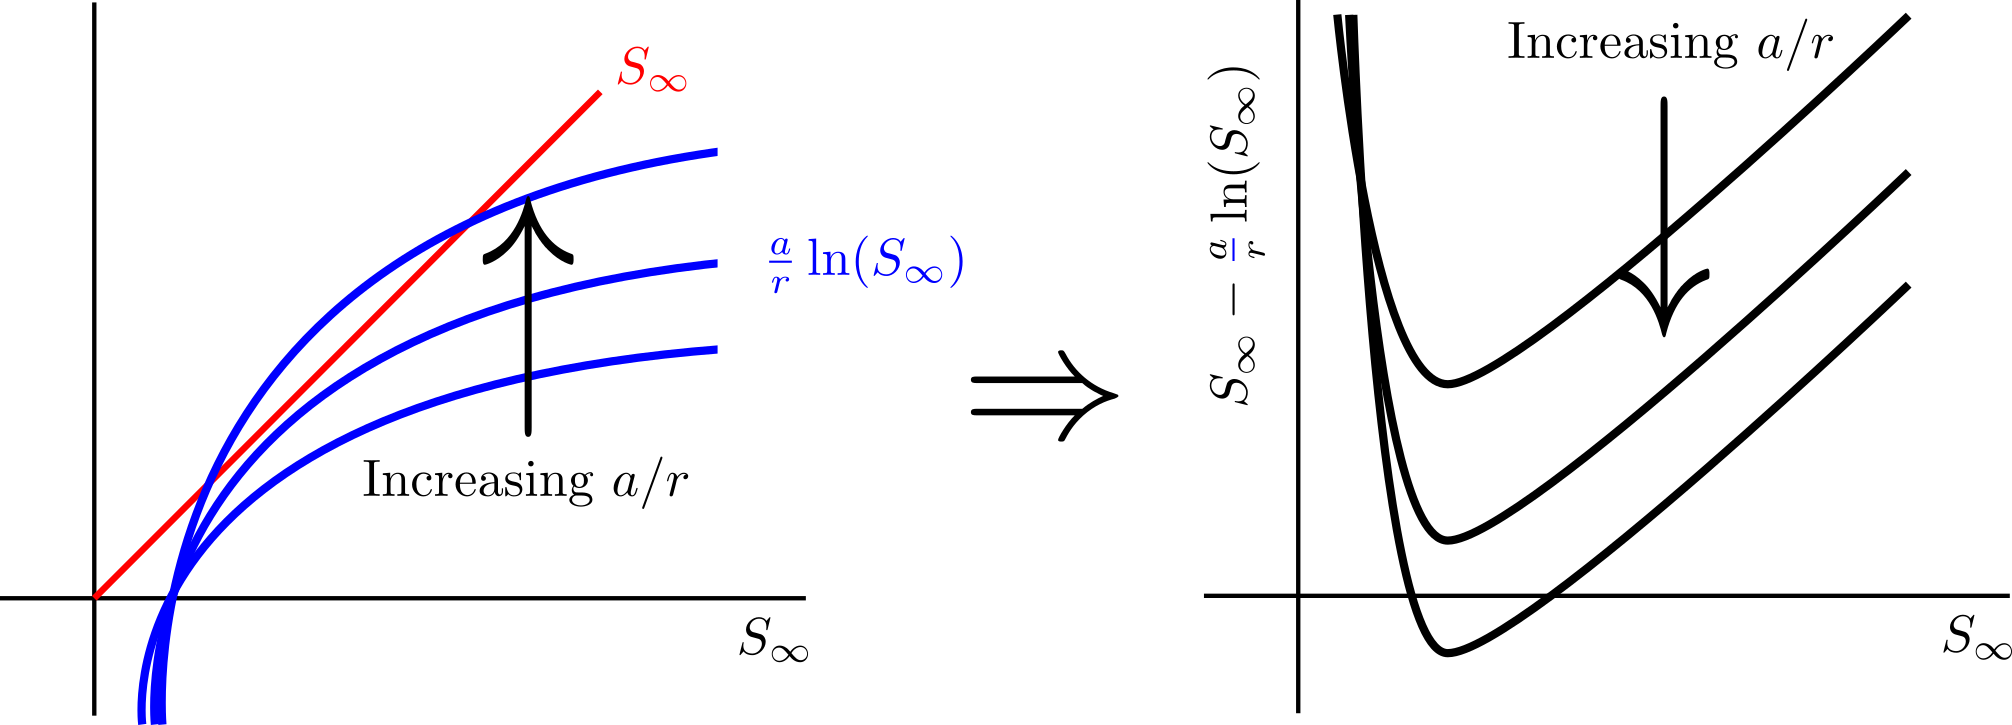
\includegraphics[width=\textwidth]{../Pictures/Infection_schematic.png}
\caption{Sketching the lines $S_\infty$ and $a\ln(S_\infty)/r$ allows us to sketch $S_\infty-a\ln(S_\infty)/r$.\label{Infection_schematic}}
\end{figure}
\begin{figure}[ph!!!tb]
\centering
\subfigure[\label{SIR_phase_plane}]{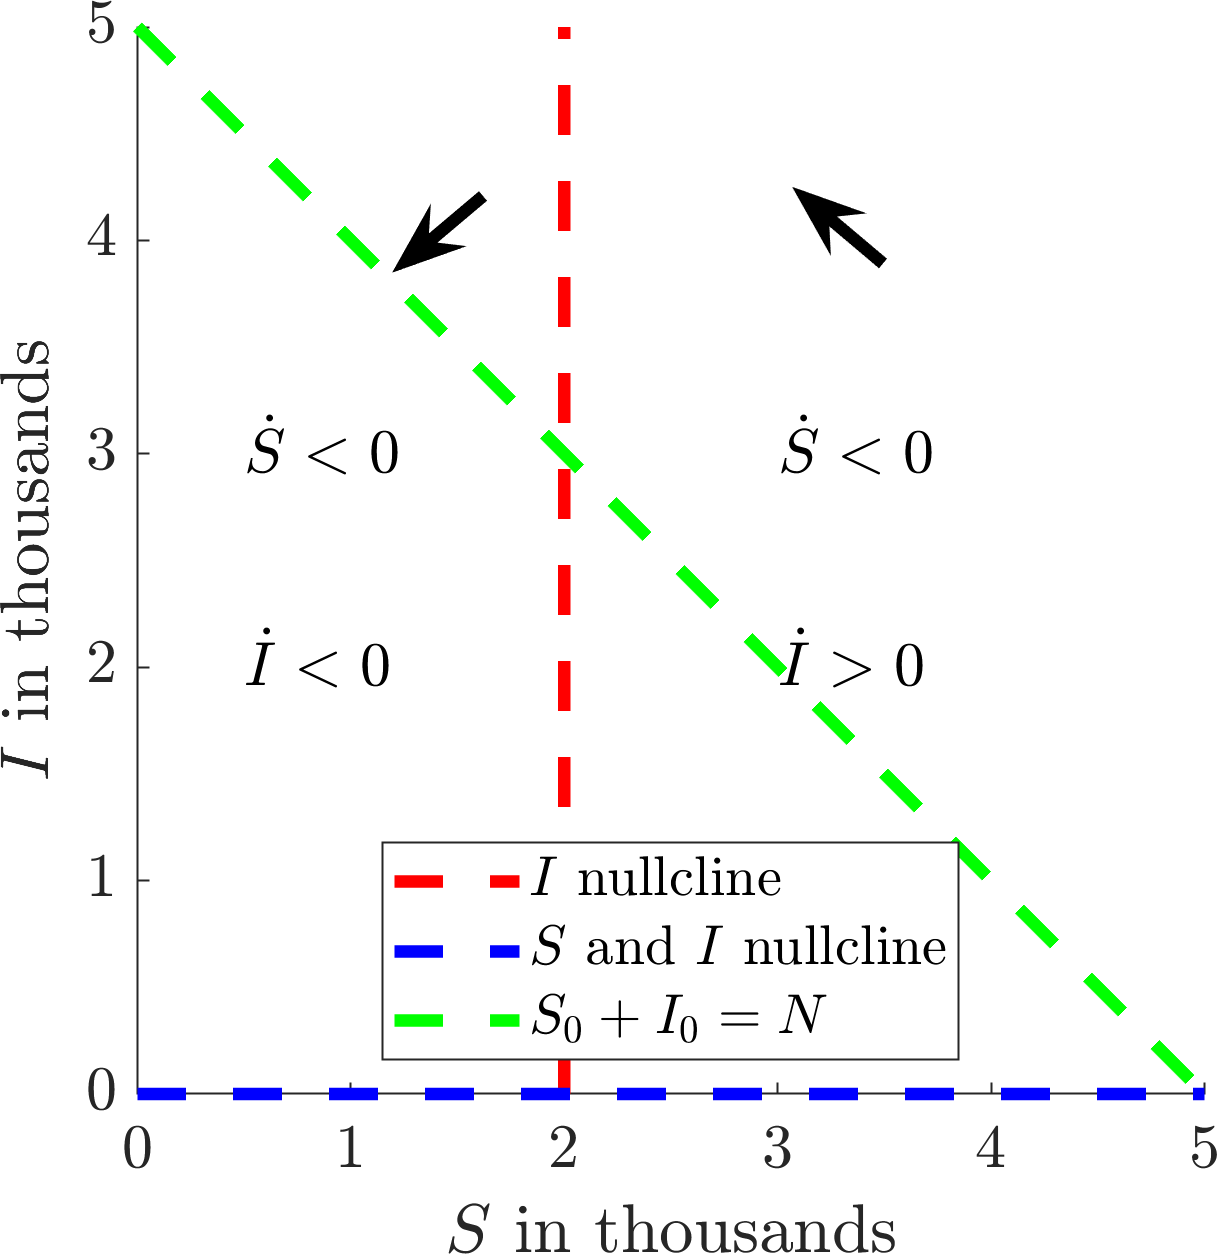
\includegraphics[height=0.35\textwidth]{../Pictures/SIR_phase_plane.png}}
\subfigure[\label{SIR_phase_plane_trajectories}]{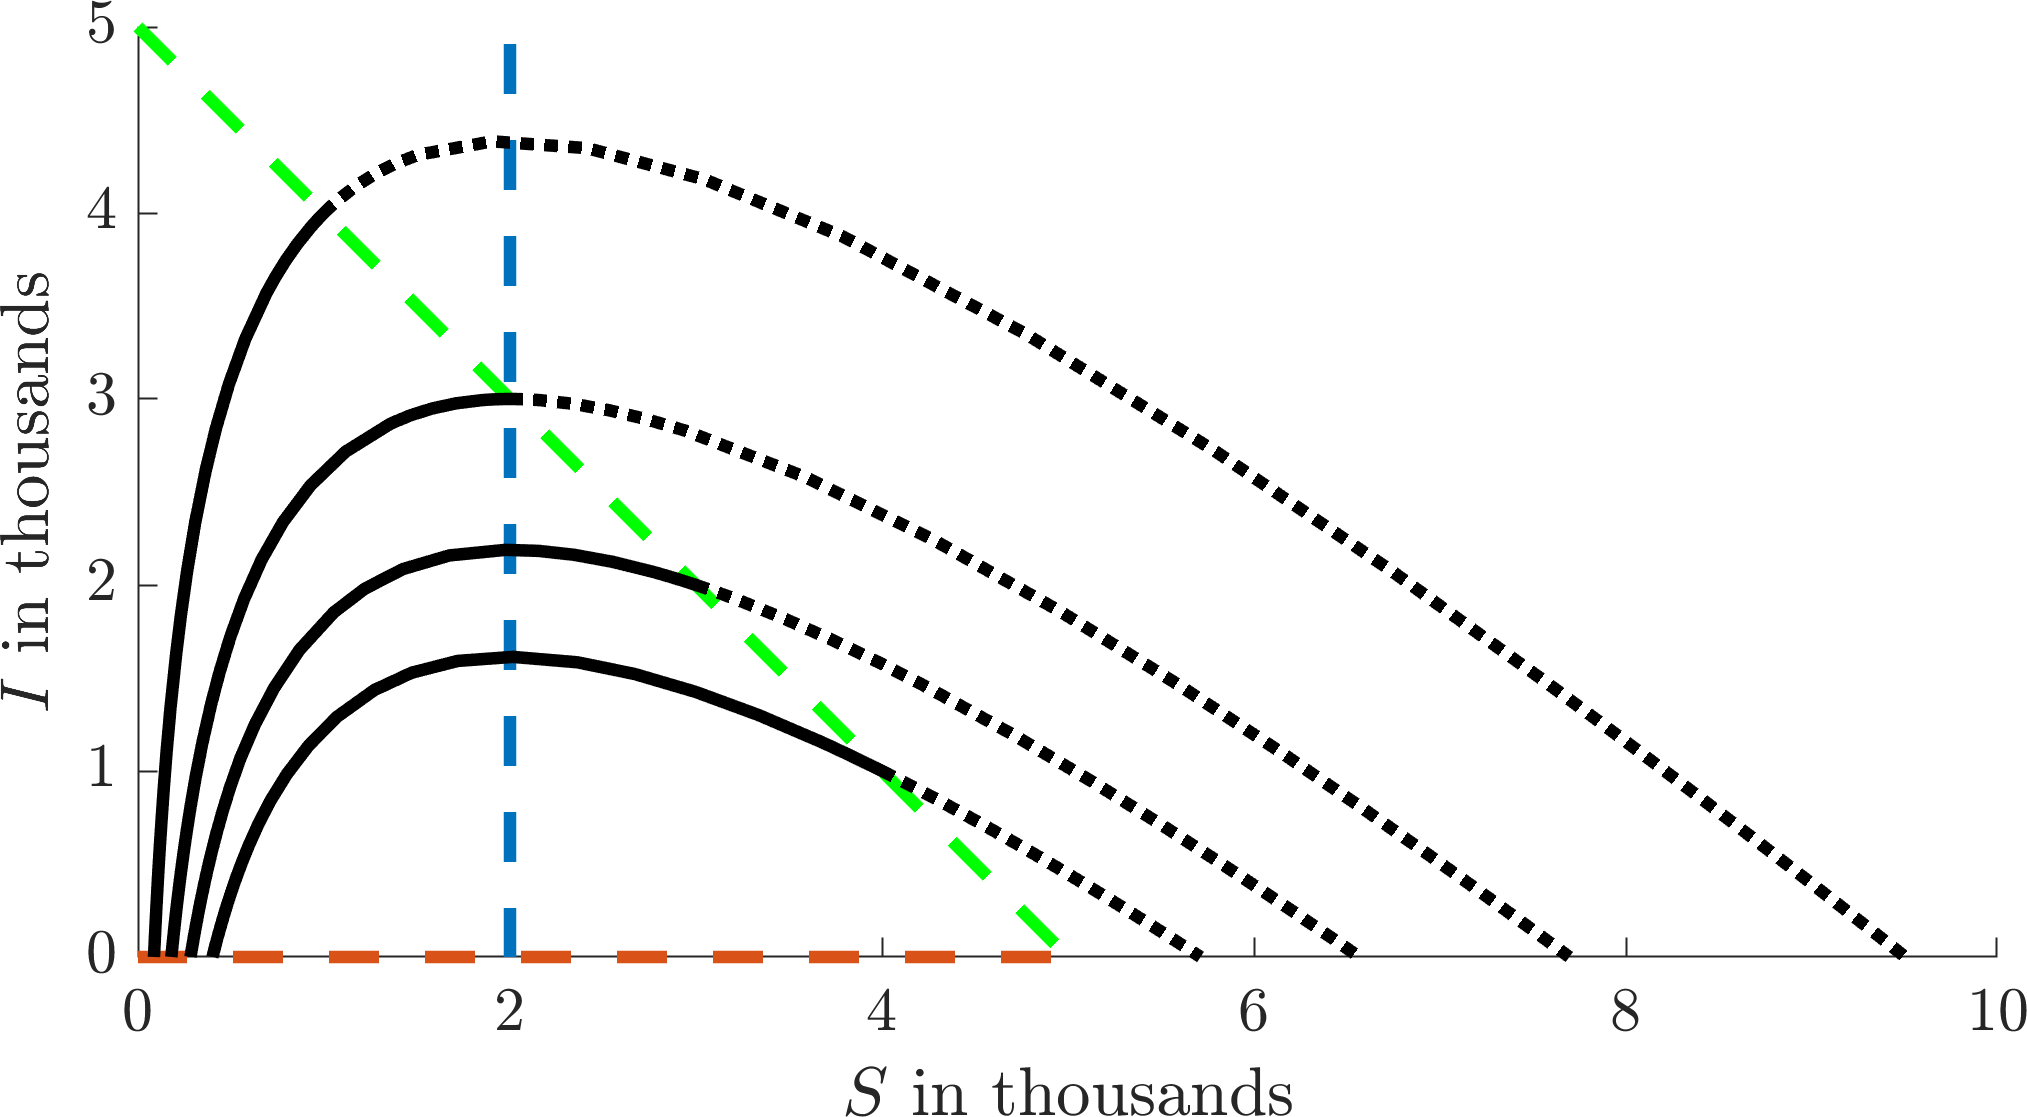
\includegraphics[height=0.35\textwidth]{../Pictures/SIR_phase_plane_trajectories.png}}
\subfigure[\label{SIR_trajectories}]{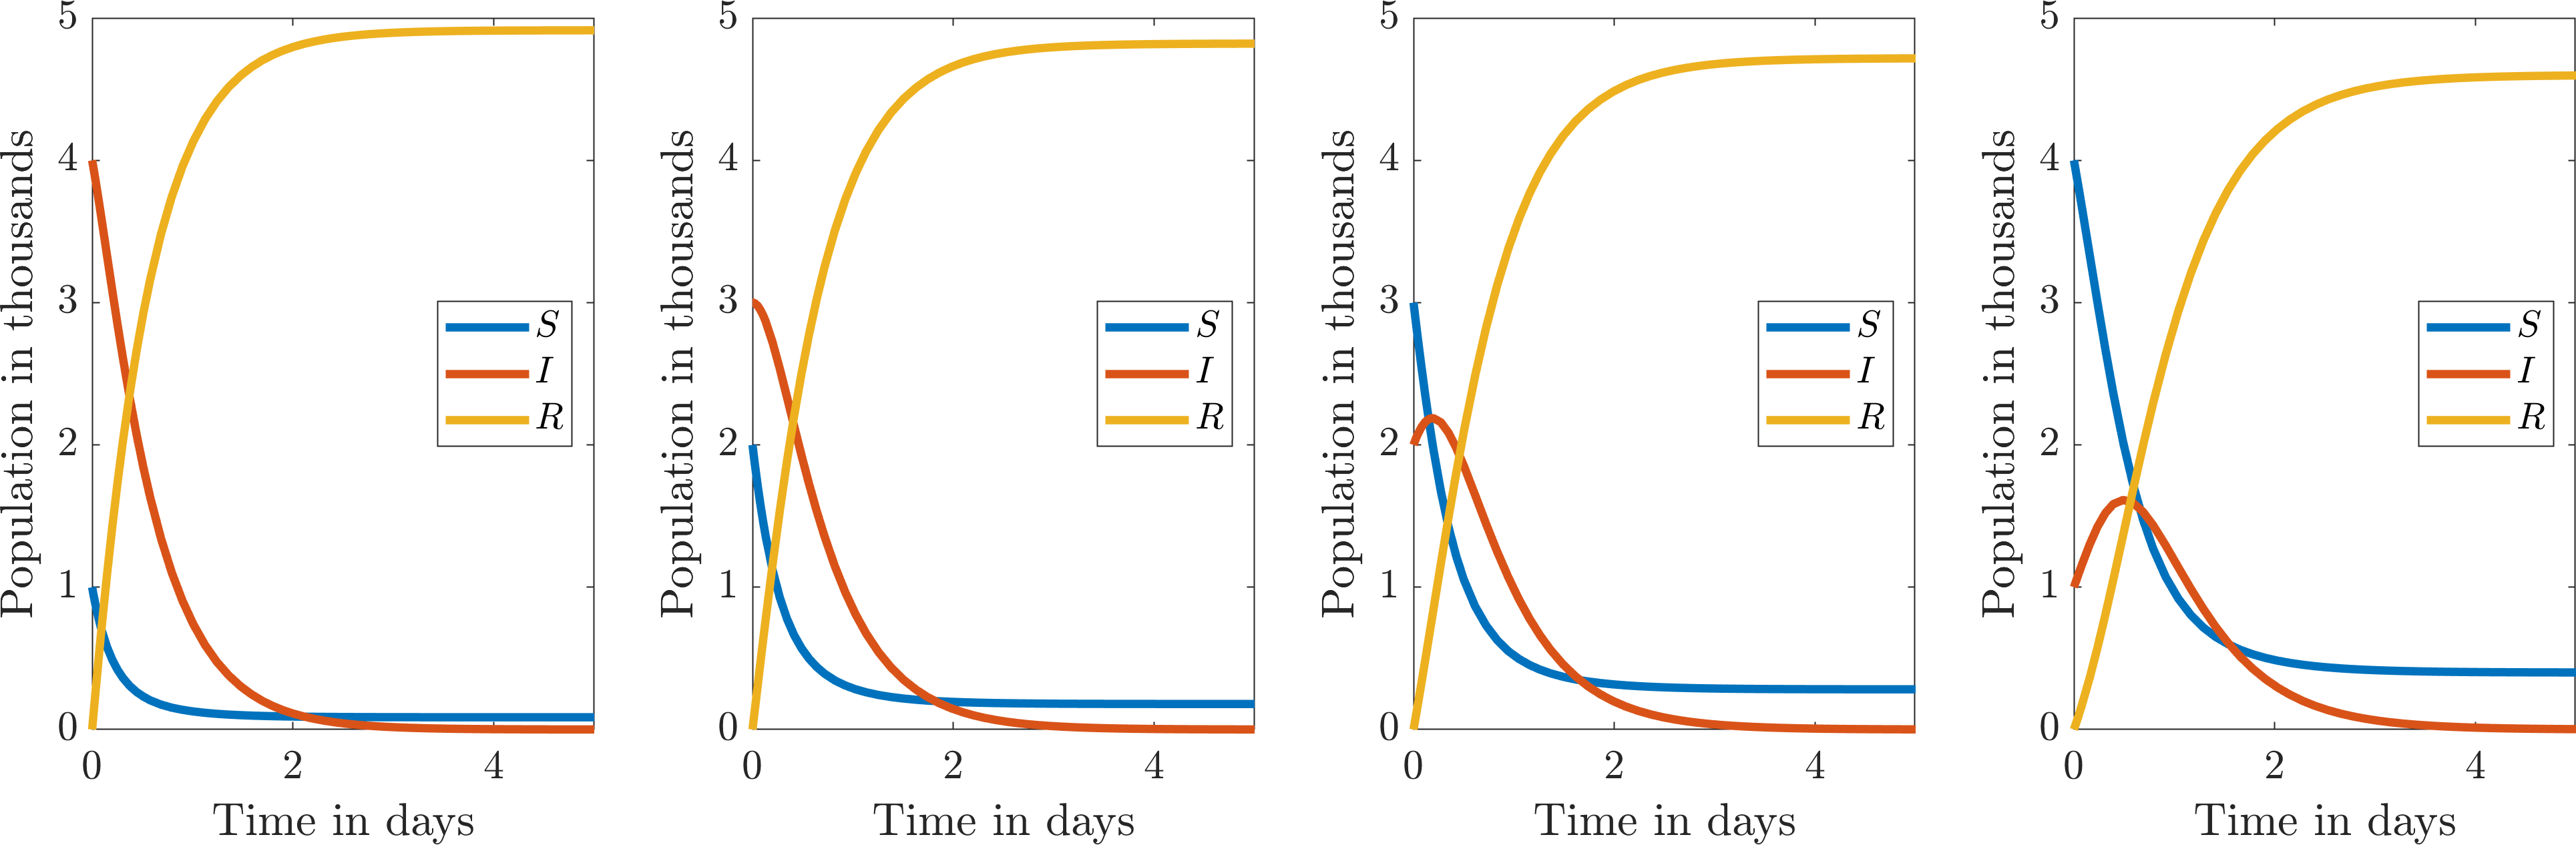
\includegraphics[width=\tp]{../Pictures/SIR_trajectories.png}}
\caption{Various methods for viewing the dynamics of the SIR system, \eqnto{S}{R} with $r=1/1000$/(person$\times$day) and $a=2$/day. The $(S,I)$ phase plane schematic is shown in (a) and is illustrated with trajectories in (b). All initial conditions are on the green dashed line and, thus, the solid lines in (b) are the forward time trajectories, whilst the dashed lines are the backward time trajectories. The four figures in (c) illustrate the $(S,I,R)$ populations of each trajectory in the (b) phase plane. The susceptible (infected) initial condition increases (decreases) left to right.}
\end{figure}

\begin{figure}[h!!!tb]
\centering
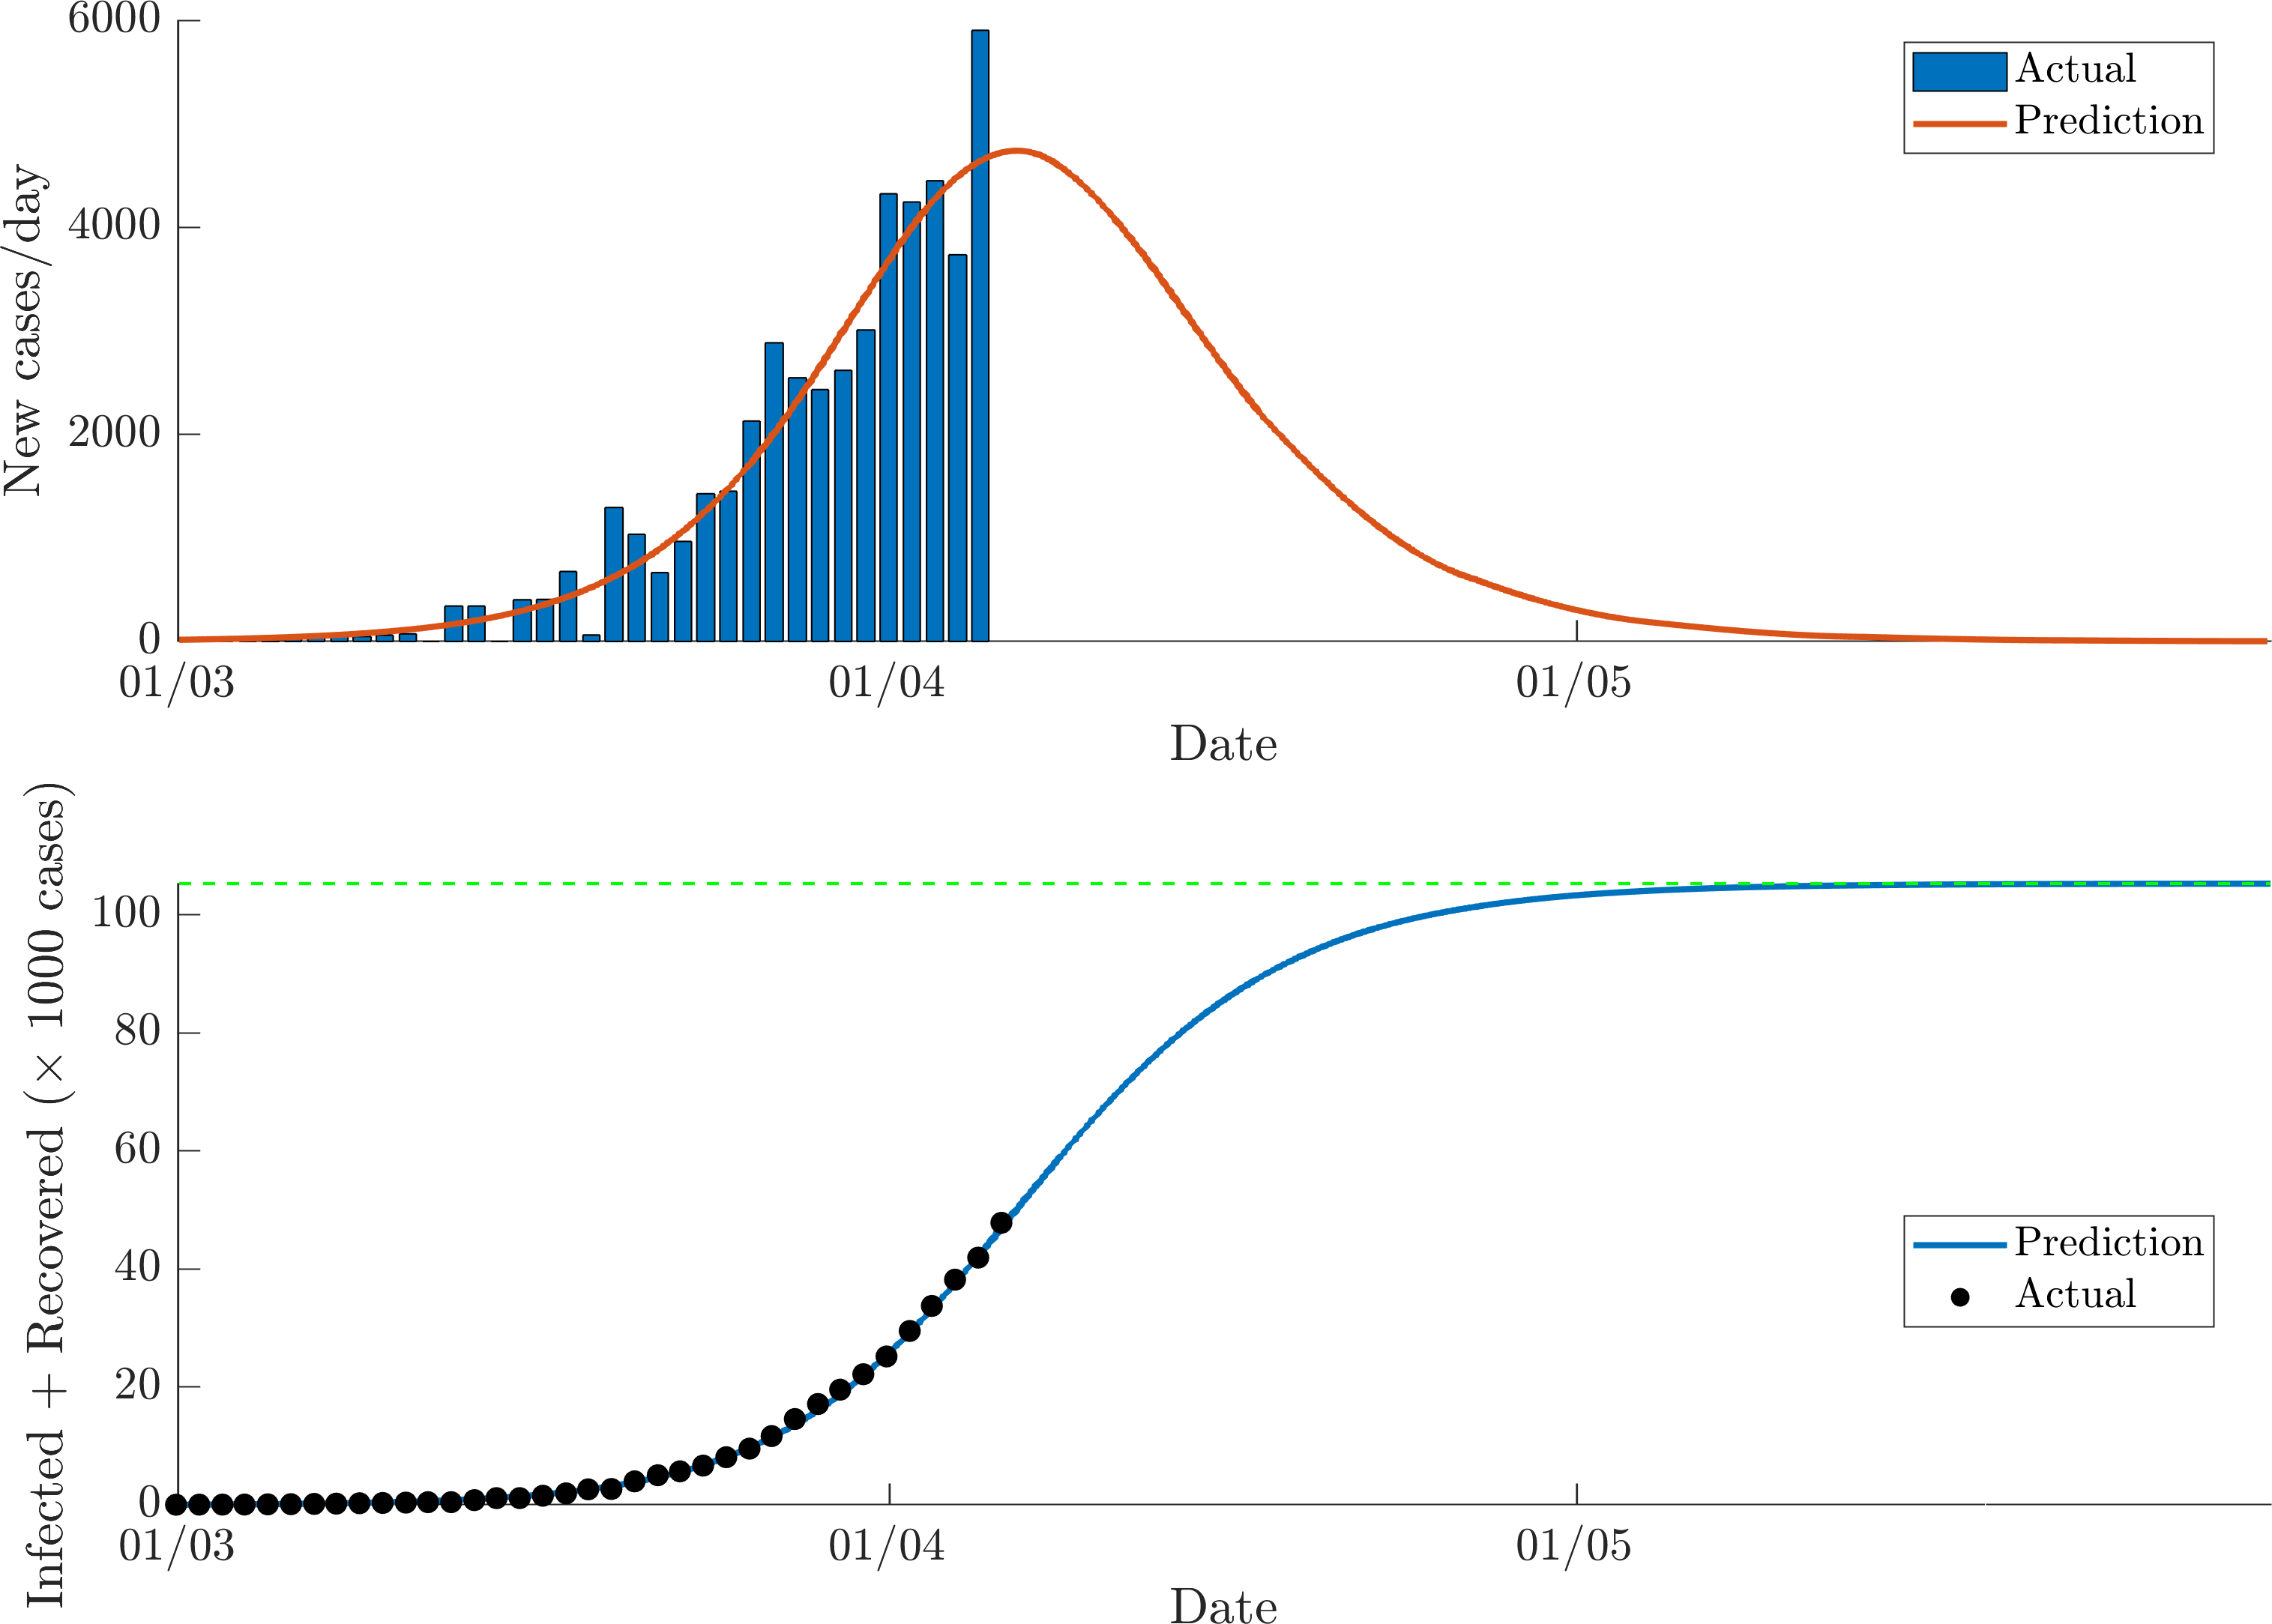
\includegraphics[width=\textwidth]{../Pictures/Covid.png}
\caption{Fitting the SIR model the the UK data of new cases from the 2020 COVID-19 pandemic between the 22nd January and 5th April. The top image shows the raw data as a bar chart. The bottom fits $I+R$ (the line) to the cumulative sum of the top data (circles). This provides estimates for the SIR parameters, which are then used to fit the prediction to the top image.\label{Covid}}
\end{figure}




\section{Discrete modelling}
ODEs are one method by which we can model populations. Critically, one of the main assumptions is that the population is dynamically changing in continuous time. This implies that there is a continuous overlap of generations. However, many species have little to no overlap between successive generations and so population growth is in discrete steps. 

For example a species of cicada known as the \textit{Magicicada neotredecim} spends almost the full length of its life underground. In the spring of their 13th year the cicadas all appear synchronously and in tremendous numbers. The cicadas develop, mate and die, such that within two months of the original emergence, their life-cycle is complete and the juvenile insects stay underground for another 13 years.

In this case, it would be pointless tracking the population in continuous time. Instead, all we would want to know is how the population at the current time depends on the population 13 years ago. Namely, we would want to construct a function $f$, such that
\bb
N_t=f(N_{t-13}).
\ee

In the models we discuss in this chapter we have scaled the time-step
to be 1. Models must thus relate the population at time $t+1$, denoted by $N_{t+1}$, in terms of the population $N_t$ at time $t$. This leads us to study difference equations, or discrete models, of the form
\bb
N_{t+1} = f(N_t),\label{General_diff}
\ee
where $f(N_t)$ is, in general, a nonlinear function of $N_t$. Such equations are usually impossible to solve analytically but again we can extract a considerable amount of information about the population dynamics without an analytical solution. 
\begin{example}[frametitle=A simple discrete population evolution \label{Discrete}]
Consider
\bb
N_{t+1}=rN_t,\quad N_0=n_0.\label{Simple_discrete}
\ee
\COL{Because \eqn{Simple_discrete} is linear we can actually provide a solution in closed form. Specifically, we simply iterate the equation back until $t=0$, \ie
\bb
N_{t+1}=rN_t=r^2N_{t-1}=r^3N_{t-2}=\dots =r^{t+1}N_0=r^{t+1}n_0.
\ee
Thus 
\bb
|N_t|\rightarrow \left\{
\begin{array}{cc}
\infty &  |r| > 1, \\
|n_0| &  |r| = 1, \\
0 &  |r| < 1. \end{array} \right. \label{Solution_simple_discrete}
\ee
Further, we note that if $r\geq 0$ the trajectories are monotonic, whereas the trajectories oscillate if $r<0$, because $r^n$ flips between positive and negative as $n$ consecutively increases.
}
\end{example}
\begin{figure}[h!!!tb]
\centering
\subfigure[\label{Simple_difference_equation_neg}]{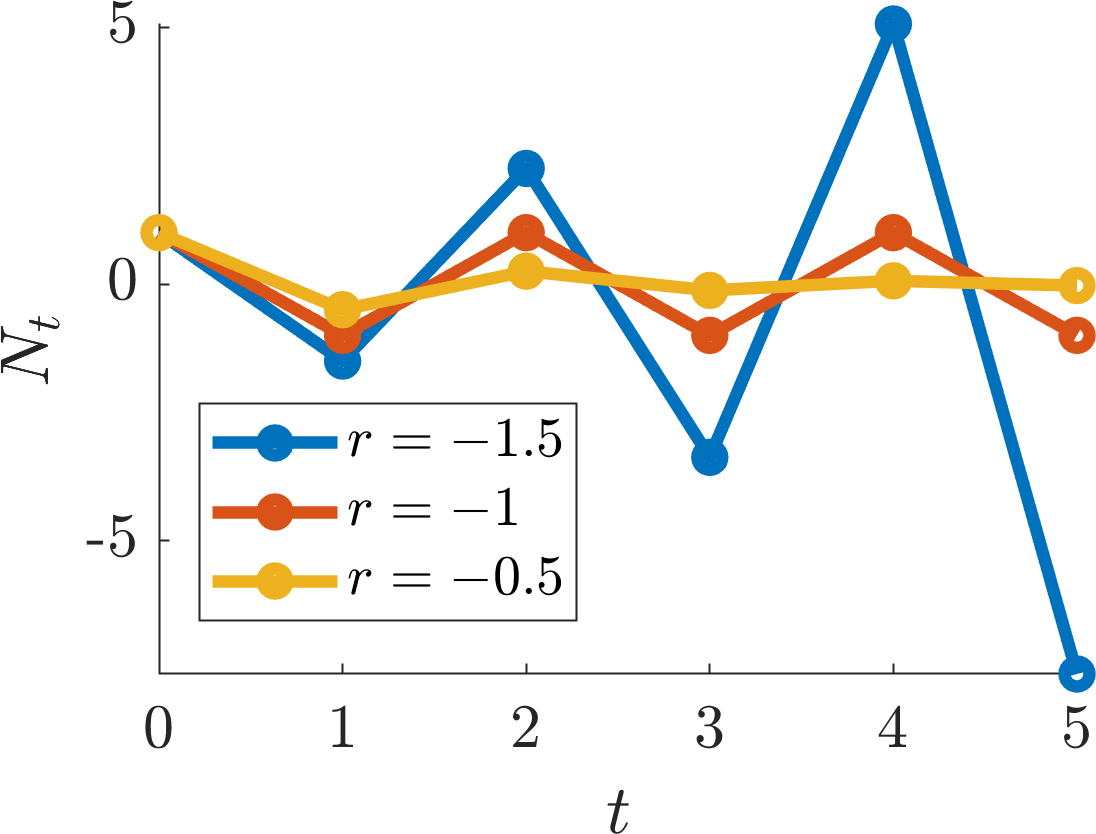
\includegraphics[width=\ttp]{../Pictures/Simple_difference_equation_neg.png}}
\subfigure[\label{Simple_difference_equation_pos}]{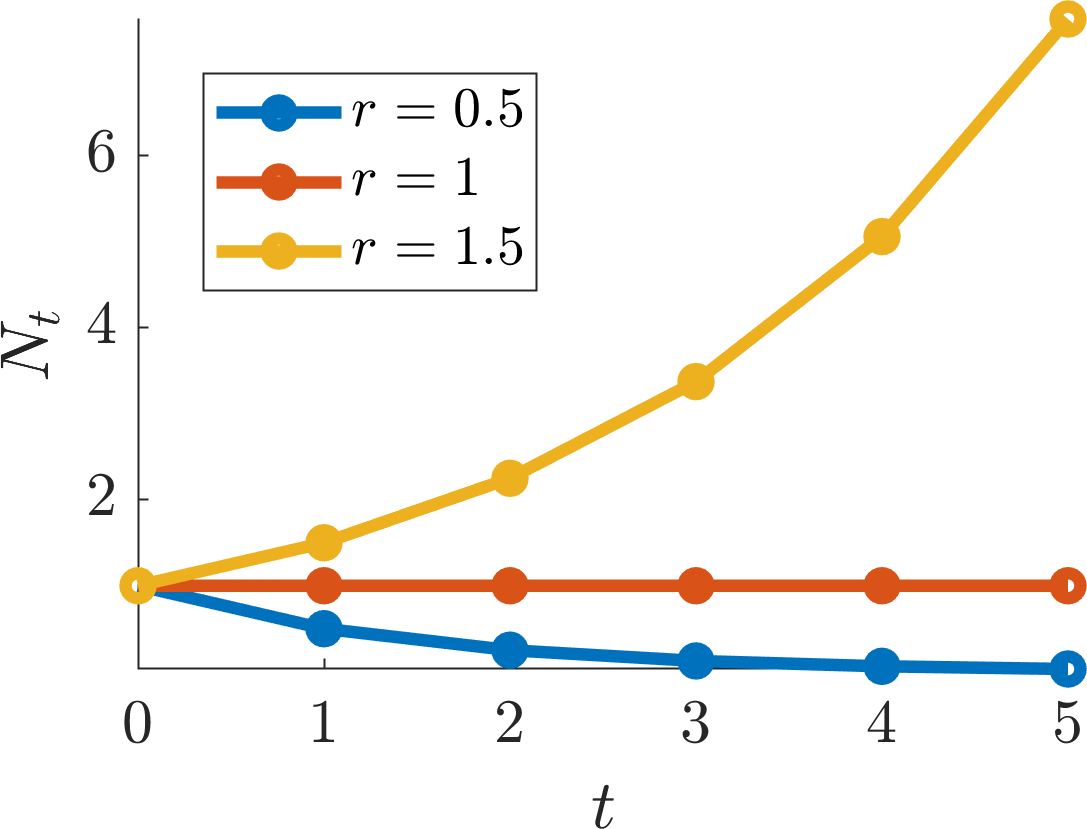
\includegraphics[width=\ttp]{../Pictures/Simple_difference_equation_pos.png}}
\caption{Plotting the solution of \eqn{Simple_discrete} with varying values of $r$. The negative values of $r$ are shown in (a), whilst the positive values are shown in (b). \label{Simple_difference_equation}}
\end{figure}

\begin{defin}
An steady state $N^*$ of a discrete population model satisfies
\bb
N^* = f(N^*).
\ee
Such points are also called fixed points, stationary points, or equilibrium points. There are analogous to ODE steady states.
\end{defin}
As you might expect, if we have a steady state then we also would like to know if it is stable or not. Namely, similar to ODEs, does a small perturbation away from $N^*$ decay to zero, or does it grow?

Before we answer this question we gain more insight into these equations through plotting their dynamics using a process called cobwebbing.

\subsection{Cobwebbing}
The dynamic evolution of $N_t$ of the general difference \eqn{General_diff} can be obtained graphically through the following algorithm.
\begin{enumerate}
\item Create a set of Cartesian axes with $N_t$ along the $x$-axis and $N_{t+1}$ along the $y$-axis.
\item Draw the diagonal line $N_t=N_{t+1}$ and sketch the function $f$, where $N_{t+1}=f(N_t)$.
\item Mark $N_0$ on the $N_t$ axis. The point $N_1$ is then given by moving vertically until we intersect the $f$ curve. Specifically, this is the point $N_1=f(N_0)$.\label{Iteration}
\item From the point $f(N_0)$ we move horizontally until we intersect the line $N_{t+1} = N_t$, which projects us onto the $N_t$-axis at $N_1$.
\item The process is repeated from line \ref{Iteration} until we can predict the future dynamics of the cobweb map.
\end{enumerate}
Critically, not only will this method provide a quick method of plotting the dynamics of population equation it also provides a means of visualising the steady states. Explicitly, the steady states are where the $N_{t+1}=f(N_t)$ curve intersects the line $N_{t+1} = N_t$.

\begin{example}[frametitle=Cobwebbing the discrete logistic equation \label{Discrete_logistic_cobwebbing}]
For a generalisation of logistic growth, consider
\bb
N_{t+1}=rN_t(1-N_t),\quad N_0=n_0.\label{Discrete_logistic}
\ee
where $0<n_0<1$. Apply the cobwebbing method to \eqn{Discrete_logistic} for different values of $r$. What happens?


\COL{We note a number of features of \eqn{Discrete_logistic}, which is cobwebbed in \fig{Logisitic_difference_simulations}:
\begin{itemize}
\item If $n_0>1$ the second iterate goes negative, thus, the model may not be useful for modelling populations in such conditions.
\item The steady states of \eqn{Discrete_logistic} are $N^*=0$ and $1-1/r$.
\item $N^*=1-1/r>0$ only makes sense when $r>1$.
\item The dynamics of the trajectories depend on $r$. Namely, \fig{Logistic_difference_equation} demonstrates that $N^*=0$ can be stable ($r<1$), or unstable ($r>1$).
\item Further, considering the top row of \fig{Logistic_difference_equation} from left to right shows that $N^*=1-1/r$ can not exist, be stable, or be unstable, respectively.
\item In the case that $r=3$, although both steady states are unstable, we have an oscillatory state.
\item If $r$ is pushed higher we can get chaotic trajectories, as seen in \fig{Logistic_difference_equation_chaos}.
\end{itemize}
}
\end{example}
\begin{figure}[ph!!!tb]
\centering
\subfigure[\label{Logistic_difference_equation}]{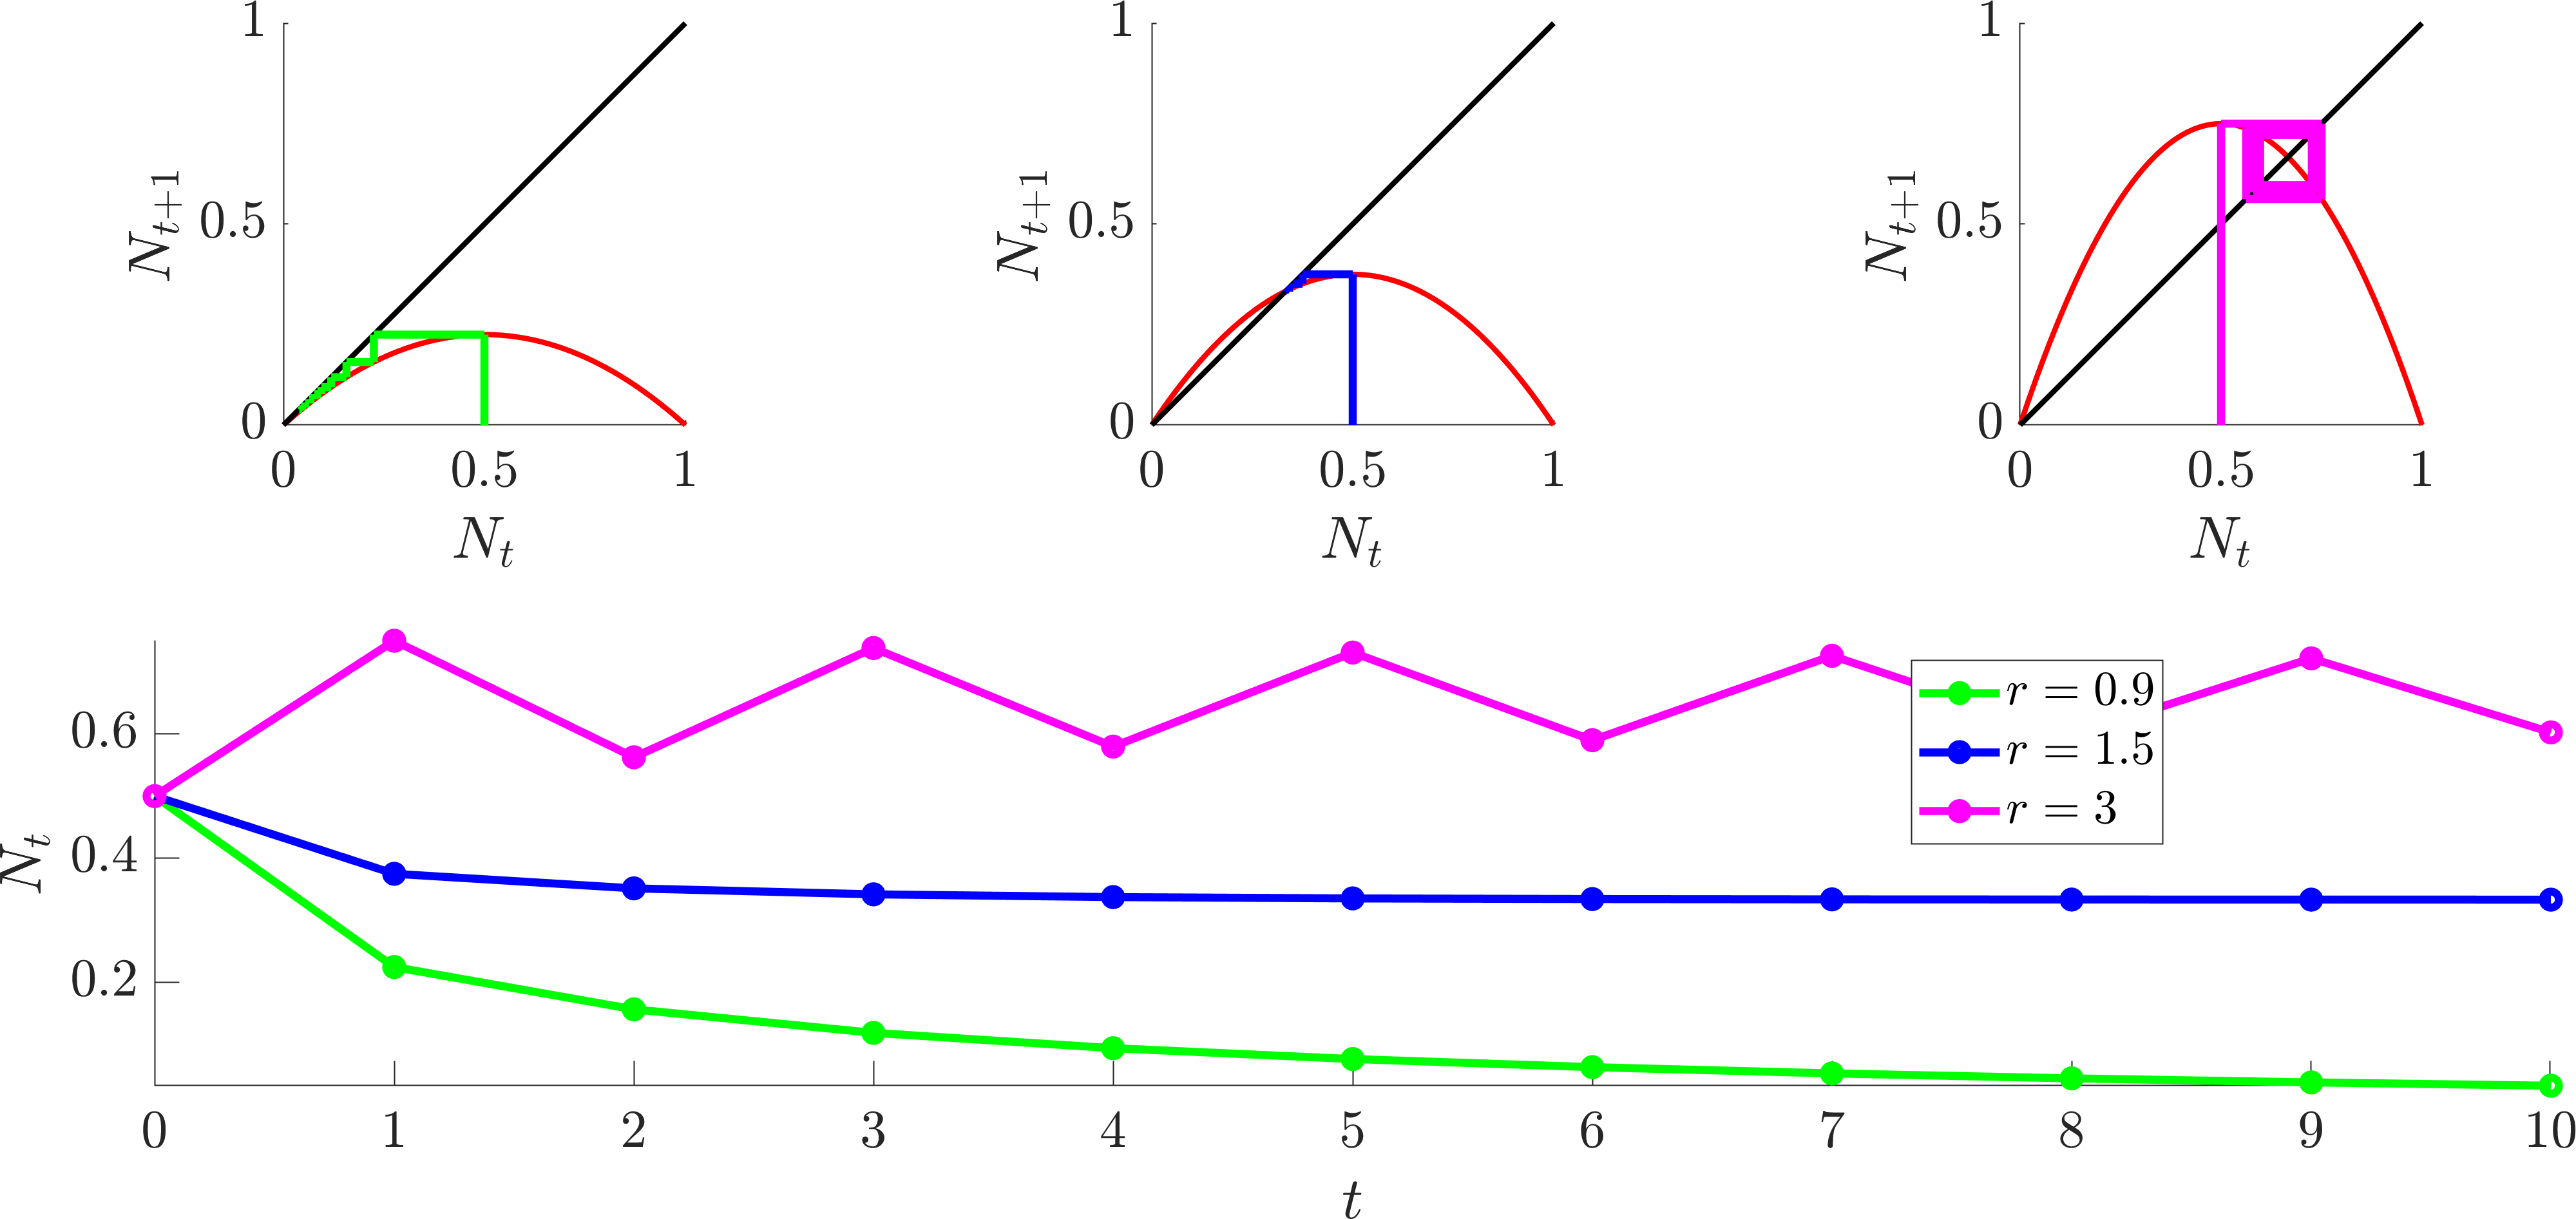
\includegraphics[width=\textwidth]{../Pictures/Logistic_difference_equation.png}}
\subfigure[\label{Logistic_difference_equation_chaos}]{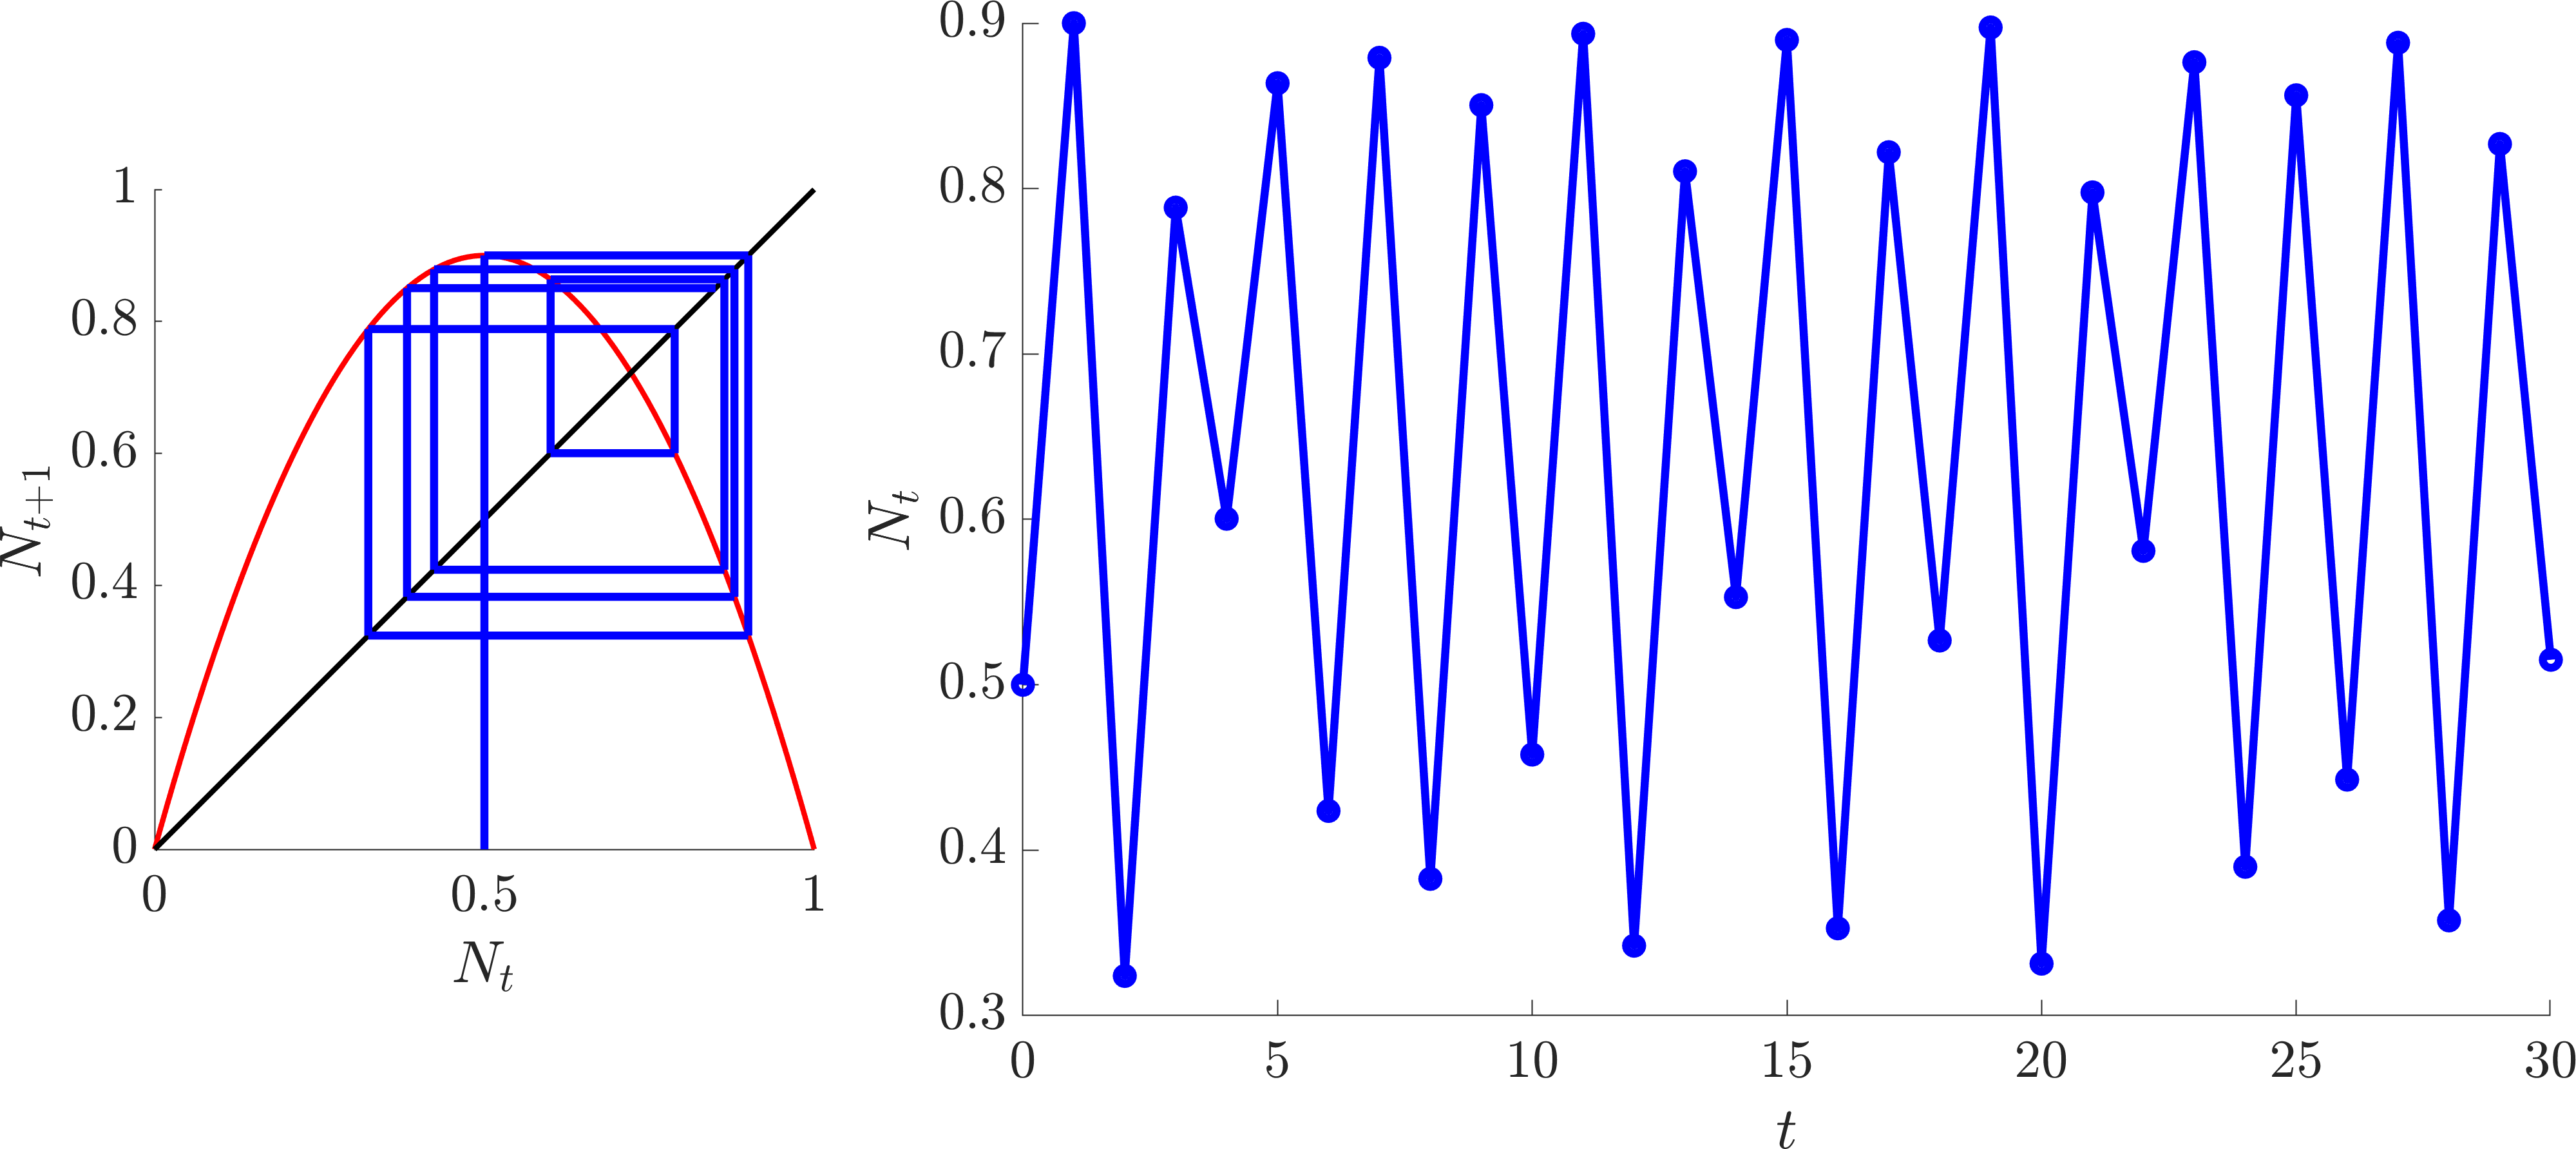
\includegraphics[width=\textwidth]{../Pictures/Logistic_difference_equation_chaos.png}}
\caption{Multiple cases of the discrete logistic equation for different values of $r$. (a) Top row, cobweb diagrams with $r=0.9, 1.5$ and 3, left to right, respectively. The accompanying trajectories are plotted in the the bottom image. (b) An example of chaotic dynamics when $r=3.6$. Left, cobweb diagram. Right, trajectory.\label{Logisitic_difference_simulations}.}
\end{figure}

\subsection{Stability of discrete equations}
Similar to continuous systems, finding steady states is only one half of the story. We would like to know whether a steady state is stable or not.
\begin{defin}
A steady state, $N^*$, of $N_{t+1}=f(N_t)$ is stable if $\forall \epsilon>0$ $\exists \delta, T>0$ such that whenever $|N_t-N^*|<\delta$ then $|N_t-N^*|<\epsilon$ $\forall t>T$. Otherwise the state is unstable.
\end{defin}

Similar to the continuous system, the proof behind the criterion for stability depends upon linearising the system. Namely, we expand the system near a steady state and ask whether a small perturbation will grow, or decay.
\begin{thm}\label{Discrete_stability}
Suppose $N^*$ is a steady state of the discrete equation
\bb
N_{t+1}=f(N_t)\label{Discrete_eqn_proof}
\ee
and assume that $f'(N^*)\neq 0$. $N^*$ is stable if $|f'(N^*)|<1$ and unstable if $|f'(N^*)|>1$. Further, near $N^*$, in either case of stability, the trajectories are monotonic if $f'(N^*)>0$ and oscillatory if $f'(N^*)<0$.
\end{thm}
\begin{proof}
\COL{Since $N^*$ is a steady state, consider the trajectory of $N_t=N^*+\epsilon_t$, where $0\leq|\epsilon_0|\ll 1$. Substituting $N_t$ into \eqn{Discrete_eqn_proof} we generate
\begin{align}
N_{t+1}&=N^*+\epsilon_{t+1},\nonumber\\
&=f(N_t),\nonumber\\
&=f(N^*+\epsilon_t).\label{Discrete_perturbation}
\end{align}
Expanding $f$ around $\epsilon_t$ gives
\bb
f(N^*+\epsilon_t)\approx f(N^*)+f'(N^*)\epsilon_t +h.o.t.\label{Discrete_approx}
\ee
and we note that $N^*=f(N^*)$, by definition. Combining \eqns{Discrete_perturbation}{Discrete_approx} gives
\bb
N^*+\epsilon_{t+1}=N^*+f'(N^*)\epsilon_t.
\ee
Thus, upon simplifying, the perturbation is governed, approximately, by
\bb
\epsilon_{t+1}=f'(N^*)\epsilon_t.
\ee
By considering example \ref{Discrete} the proof is complete. Explicitly, the size of the perturbation, $|\epsilon_t|$, grows if $|f'(N^*)|>1$, meaning that $N^*$ is unstable. Alternatively,  $|\epsilon_t|$, shrinks if $|f'(N^*)|<1$, meaning that $N^*$ is stable. Equally, the trajectories are monotonic (oscillate) in the case that $f'(N^*)>0$ ($f'(N^*)<0$). Note that this is only true in the $\epsilon$ expansion around the steady state.}
\end{proof}
\begin{example}[frametitle=Discrete logistic equation revisited \label{Discrete_logistic_revisited}]
As noted in example \ref{Discrete_logistic_cobwebbing} the steady states of the discrete logistic equation are $N^*=0$ and $1-1/r$. Suppose we only consider the case when $r>0$. Characterise the linear stability of the two steady states.

\COL{As stated in Theorem \ref{Discrete_stability} we need to consider the derivative of $f(N)=rN(1-N)$ at the steady states. Specifically, $f'(N)=r-2rN$, thus, $f'(0)=r$ and $f'(1-1/r)=2-r$. Hence, the steady state $N^*=0$ always exists, but is only stable for $-1<r<1$. Since $r>0$ by restriction we have that $N^*=0$ is stable $0<r<1$ and unstable when $r>1$. 

$N^*=1-1/r$ only exists when $r\geq 1$ and is stable only when $|2-r|<1$,
\begin{align}
1>&|r-2|,\nonumber\\
\implies 1>&r-2>-1,\nonumber\\
\implies 3>&r>1.\nonumber
\end{align}
Combining all these inequalities, we see that $N^*=1-1/r$ exists and is stable for $1<r<3$ and }\COL{is unstable when $r>3$. All of this information can be illustrated in a bifurcation diagram, as seen in \fig{Logistic_bifurcation_diagram}.}
\end{example}
\begin{figure}[ph!!!tb]
\centering
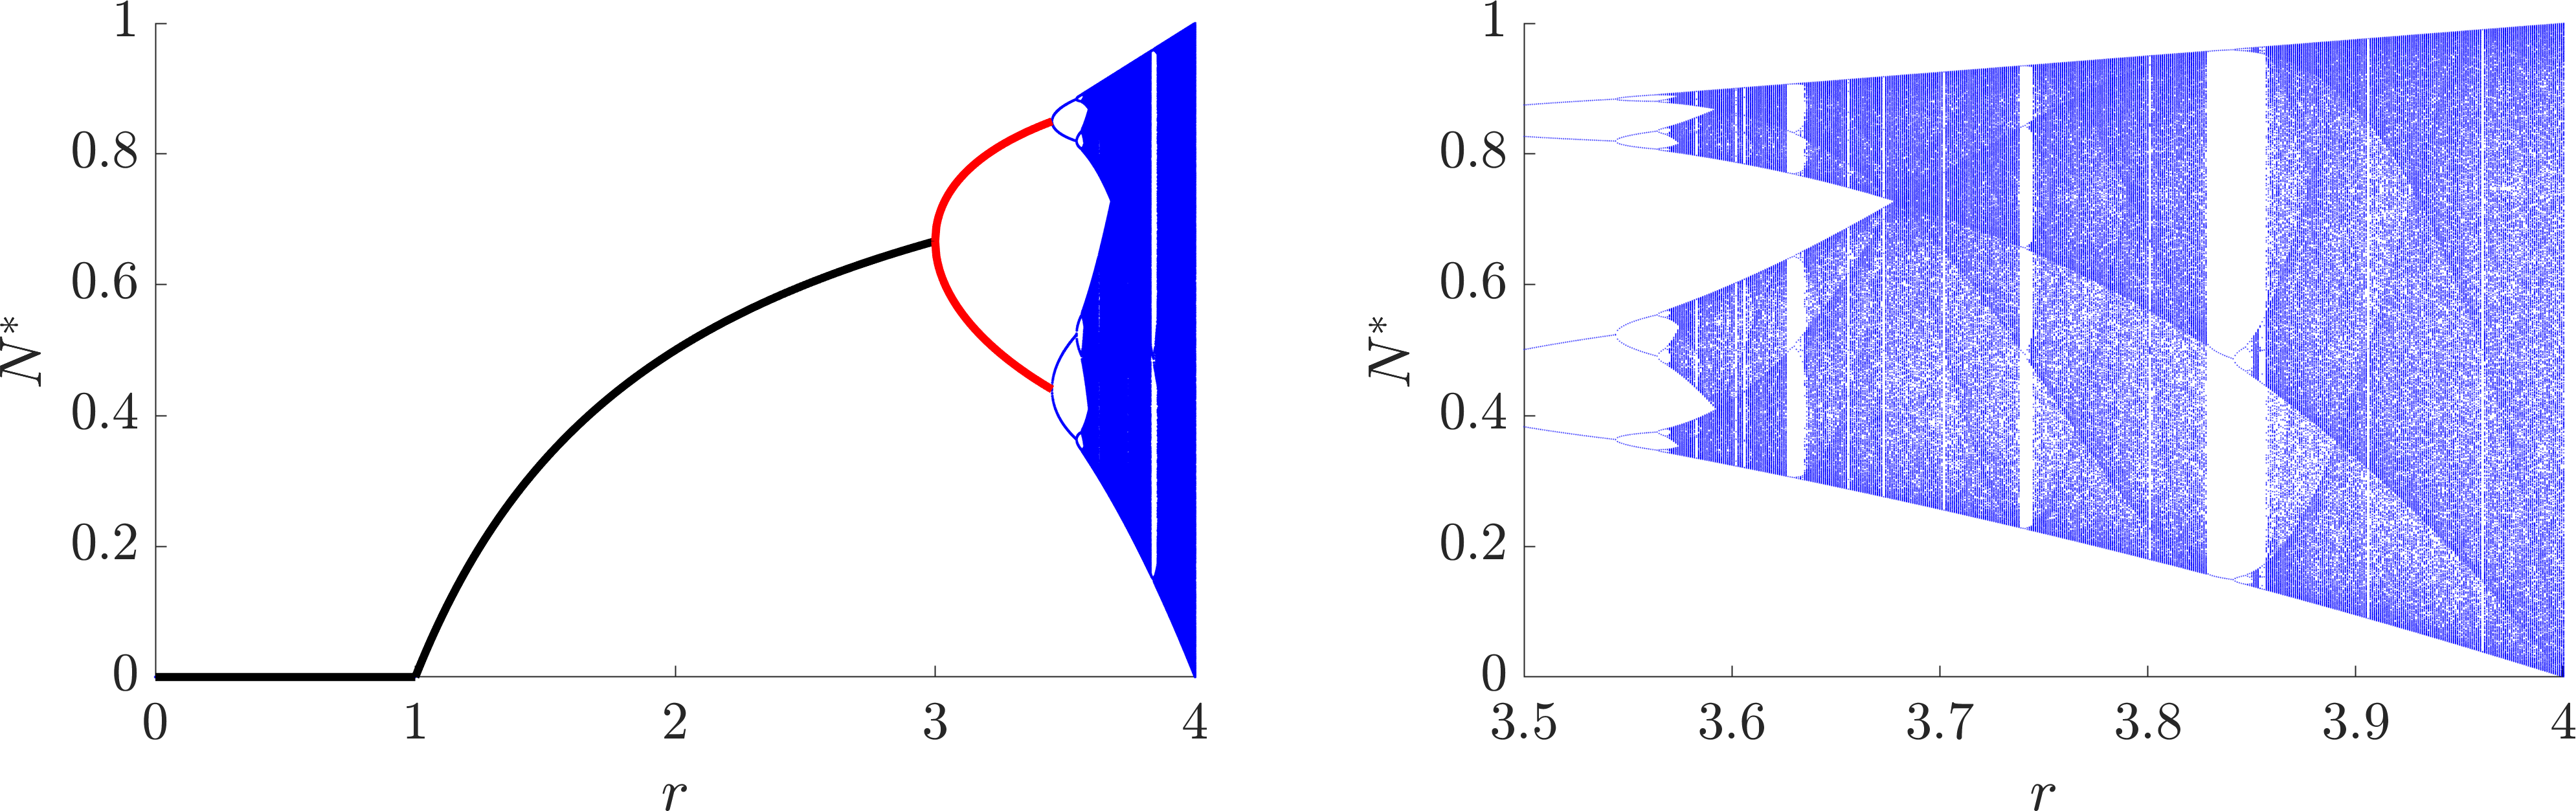
\includegraphics[width=\textwidth]{../Pictures/Logistic_bifurcation.png}
\caption{Bifurcation diagram of the discrete logistic equation \eqref{Discrete_logistic}. On the left we see the derived regions of stability for $N^*=0$ and $1-1/r$ (black line) from example \ref{Discrete_logistic_revisited}. In example \ref{Discrete_logistic_oscillations} we will also derive the values and region of stability of the period 2 oscillatory states (red line). However, the derivation of the activity in the blue region is outside the scope of the course, although we can simulate it easily. The right image shows a magnification of the region $3.5<r<4$, which illustrates that the discrete logistic system can produce a chaotic trajectory.\label{Logistic_bifurcation_diagram}}
\end{figure}

\subsection{Oscillatory states in discrete equations}
\begin{defin}
We define the $p^{th}$ iterate of a map to be the $p$th time step. Namely
\bb
f^p(N_t)=\underbrace{f(f(\dots f}_{\textrm{p times}}(N_t)\dots))=N_{t+p}.
\ee
\end{defin}
\begin{defin} A state, $N^*$, has an oscillatory period $p$ if $p$ is the smallest integer such that $N^*=f^p(N^*)$.
\end{defin}
\begin{thm}
Suppose $N_{t+1}=f(N_t)$ has a oscillatory point, $N^{1*}$, of period $p$. Then there are also $p-1$ distinct points that have oscillatory period $p$.
\end{thm}
\begin{proof}
\COL{Consider the points $N^{1*}, N^{2*}=f(N^{1*}),N^{3*}=f(N^{2*})=f^2(N^{1*}),\dots,N^{p*}=f(N^{(p-1)*})=f^{(p-1)}(N^{1*})$. By assumption $N^{1*}=f(N^{p*})$ and by definition
\bb
f^p(N^{i*})=f^p(f^{i-1}(N^{1*}))=f^{i-1}(f^{p}(N^{1*}))=f^{i-1}(N^{1*})=N^{i*}
\ee
for all $1\leq i\leq p$. Thus, $N^{i*}$ does evaluate to itself after $p$ iterations. Finally, we have to show that $f^q(N^{i*})\neq N^{i*}$ for $q<p$. For a contradiction suppose that for some $1<i\leq p-1$ there does exist $q<p$ such that $f^q(N^{i*})=N^{i*}$. Then
\bb
f^{p+1-i}(f^q(N^{i*}))=f^{p+1-i}(N^{i*}),
\ee
but
\bb
f^{p+1-i}(N^{i*})=f^p(N^{1*})=N^{1*}
\ee
and
\bb
f^{p+1-i}(f^q(N^{i*}))=f^{p+q}(N^{1*})=f^{q}(N^{1*}).
\ee
However, by definition $f^{q}(N^{1*})\neq N^{1*}$ for $q<p$. Hence, by contradiction the proof is complete.}
\end{proof}
\begin{defin}
The orbit of an oscillatory point, $N^{1*}$ with period $p$, of a map $f$, is the set of points $\{N^{1*}, N^{2*}=f(N^{1*}),N^{3*}=f(N^{2*})=f^2(N^{1*}),\dots,N^{p*}=f(N^{(p-1)*})=f^{(p-1)}(N^{1*})\}$.
\end{defin}
As seen in \figs{Logistic_difference_equation}{Logistic_bifurcation_diagram}, when $r$ increases past 3 there is no longer a single steady state. Rather the system undergoes a bifurcation to an oscillatory trajectory of period 2. Further, \fig{Logistic_bifurcation_diagram} shows that around $r\approx 3.5$ the system bifurcates again into a period 4 oscillation. As $r$ increases further a cascade of bifurcations happen leading to states with higher periods of oscillations, demonstrating that that the discrete logistic system can produce chaotic trajectories.

As you might expect, understanding the full chaotic region is extremely complicated. However, we can move beyond just the steady states to consider the simple oscillatory states. For example, suppose a system has a period 2 oscillation, \ie there are two (non-equal) states, $N^*_1$ and $N^*_2$, such that $N^*_1=f(N^*_2)$ and $N_2^*=f(N_1^*)$. Each state is then a steady state of $f^2$, \ie
\bb
f^2(N_1^*)=f(f(N_1^*))=f(N_2^*)=N^*_1.
\ee
\begin{thm}\label{Oscillation_theorem}
If $N^*$ is an oscillatory state of $f$, of period $p$, it is a steady state of $f^p$.
\end{thm}
\begin{proof}
Practically by definition.
\end{proof}
\begin{thm}\label{Discrete_theorem}
Suppose $N^*$ is an oscillatory state of period $m$, where $m$ is a factor of $p$ then $N^*$ is also a steady state of $f^p$.
\end{thm}
\begin{proof}
\COL{By definition $N^*=f^m(N^*)$ and by assumption there exists a positive integer $n$ such that $p=mn$. Hence
\begin{align}
f^p(N^*)&=f^{mn}(N^*),\nonumber\\
&=\underbrace{f^{m}(f^m(\dots f^m}_{\textrm{n times}}(N^*)\dots)),\nonumber\\
&=N^*.\nonumber
\end{align}}
\end{proof}
From theorems \ref{Oscillation_theorem} and \ref{Discrete_theorem} we have a way of finding periodic states. From stability theorem \ref{Discrete_stability} we also have a way of characterising the stability of a period $p$ oscillation, namely, $x_p$ is a stable period $p$ oscillation of the map $f$ if $x_p$ is a stable state of the map $f^p$. Explicitly,
\bb
x_p \textrm{ is }
\left\{\begin{array}{l}
\textrm{ stable if }\left|\frac{\rd f^p (x_p)}{\rd x}\right|<1,\\
\textrm{ unstable if }\left|\frac{\rd f^p (x_p)}{\rd x}\right|>1.
\end{array}\right.
\ee
However, calculating $\rd f^p (x_p)/\rd x$ often requires difficult algebraic manipulations. Thankfully, the following theorem simplifies the issue.
\begin{thm}\label{Map_derivative}
Let $x^{1*}$ be a period $p$ oscillation of $f$ then
\bb
\frac{\rd f^p (x^{1*})}{\rd x}=f'(x^{1*})f'(x^{2*})f'(x^{3*})\dots f'(x^{p*}),
\ee
where $x^{i*}=f^{i-1}(x^{1p})$.
\end{thm}
\begin{proof}
\COL{By the chain rule if $g(x)$ and $h(x)$ are two well-behaved functions with derivatives $g'(x)$ and $h'(x)$, respectively, then
\bb
\frac{\rd g(h(x))}{\rd x}=g'(h(x))h'(x).
\ee
Applying this iteratively to $f^{p}(x)=f(f(\dots f(x)\dots ))$ we derive
\bb
\frac{\rd f^p(x)}{\rd x}=f'(x)f'(f(x))f'(f^2(x))\dots f'(f^{p-1}(x)).\label{Chain_rule_evaluation}
\ee
Evaluating \eqn{Chain_rule_evaluation} at $x=x^{1*}$ provides the required result.}
\end{proof}
Thus, instead of evaluating the derivative of the $p$th iteration map we need only calculate the derivative of the original map and evaluate it at all period $p$ steady states. This evaluation may not be easier, but it should be easier that evaluating the derivative of the $p$th iteration map. This also then leads to the following observation
\begin{cor}
The stability of all periodic points in the same orbit is the same, namely,
\bb
\frac{\rd f^p(x^{1*})}{\rd x}=\frac{\rd f^p(x^{2*})}{\rd x}=\dots=\frac{\rd f^p(x^{p*})}{\rd x}.
\ee
\end{cor}
\begin{proof}
\COL{By considering \eqn{Chain_rule_evaluation} and noting that $f^i(x^{j*})=f(x^{(i+j)*})$ we can see the right-hand side of $\rd f^p(x^{j*})/\rd x$ will be just be permutation of the terms of $\rd f^p(x^{1*})/\rd x$. Thus, the product will be the same.}
\end{proof}
\begin{example}[frametitle=Period 2 oscillations in the discrete logistic equation \label{Discrete_logistic_oscillations}]
Derive the period two oscillation states specifying their existence and stability dependence on $r$.


\COL{Using the insights from the above discussion and theorems to extract the period 2 oscillatory states we need to consider the second iteration of the discrete logistic equation. Namely, if
\bb
N_{t+1}=rN_t(1-N_t)=f(N_t)\nonumber
\ee
then we need to consider the steady states of $f^2$. Since $f$ is a quadratic then $f^2$ will be a quartic. These are difficult to solve. However, by Theorem \ref{Discrete_theorem} we know two of the roots. Namely, the steady states of $f$ ($N^*=0, 1-1/r$) will also be steady states of $f^2$. Since we know two roots, we can factor these out of the quartic, leaving only a quadratic needing to be factored, which we can easily work with.

Thus, we need to consider the steady states of $f^2$,
\begin{align}
N=f^2(N)&=f(f(N)),\nonumber\\
&=rf(N)(1-f(N)),\nonumber\\
&=r[ rN(1-N)](1-[ rN(1-N) ]),\nonumber\\
&=r^2N(1-N)(1- rN(1-N) ). \label{Discrete_period_2}
\end{align}
Rearranging \eqn{Discrete_period_2} and factoring the $N^*=0$ root gives
\begin{align}
0&=N(r^2(1-N)(1- rN(1-N) )-1),\nonumber\\
&=N(r^2(1-N)(1- rN+rN^2 )-1),\nonumber\\
&=N(r^2(1- rN+rN^2-N+ rN^2-rN^3 )-1),\nonumber\\
&=N(r^2-1- r^2(r+1)N+2r^3N^2-r^3N^3 ).\label{Period_2_factor_1}
\end{align}
As mentioned, we further know that $1-1/r$ is a root, meaning that there are some values of $a,b$ and $c$ such \eqn{Period_2_factor_1} has the following form
\begin{align}
0&=N(N-[1-1/r])(a+bN+cN^2),\label{General_quadratic}\\
&=N(-a(r-1)/r+(ar-br+b)N/r+(br-cr+c)N^2/r+cN^3)\label{General_cubic}.
\end{align}
Comparing \eqns{Period_2_factor_1}{General_cubic} we immediately see that
\bb
a=-\frac{(r^2-1)r}{r-1}=-(r+1)r \textrm{ and } c=-r^3.\label{Discrete_a_c}
\ee
}\COL{and
\begin{align}
2r^3&=\frac{br-cr+c}{r},\nonumber\\
&=\frac{br+r^4-r^3}{r},\nonumber\\
&=b+r^3-r^2,\\
\implies b&=r^2+r^3=r^2(1+r).\label{Discrete_b}
\end{align}
Substituting \eqns{Discrete_a_c}{Discrete_b} into \eqn{General_quadratic} we generate
\bb
0=N(N-[1-1/r])(-r(r+1)+r^2(1+r)N-r^3N^2).
\ee

Thus, the period two steady states satisfy
\begin{align}
0&=-r(r+1)+r^2(1+r)N-r^3N^2.\nonumber\\
0&=r^2N^2-r(1+r)N+(r+1).\label{Quad_relationship}\\
\implies N^\pm&=\frac{r(1+r)\pm\sqrt{r^2(1+r)^2-4r^2(r+1)}}{2r^2},\nonumber\\
&=(1+r)\frac{1\pm\sqrt{1-4/(r+1)}}{2r}.\label{Oscillatory_roots}
\end{align}
Critically, we must have $1-4/(r+1)>0$ for the states to be valid \ie $r>3$. Hence, these states appear as the $N^*=1-1/r$ destabilize. But are they stable? To answer this question we must consider the size of
\bb
{f^2}'(N^\pm)=\frac{\rd}{\rd N}\l r^2N(1-N)(1- rN(1-N) )\r|_{N=N^\pm}.
\ee
The above derivative could be calculated, but we will use Theorem \ref{Map_derivative}. Namely
\bb
{f^2}'(N^\pm)=f'(N^+)f'(N^-).
\ee
We have already calculated $f'=r-2rN$ in example \ref{Discrete_logistic_revisited}, so,
\begin{align}
{f^2}'(N^\pm)=&r^2(1-2N^+)(1-2N^-),\nonumber\\
=&r^2(1-2(N^++N^-)+4N^+N^-),\nonumber\\
=&r^2\l 1-2\frac{(1+r)}{r}+4\frac{r+1}{r^2} \r,\nonumber\\
=&-r^2+2r+4.
\end{align}

For stability we need $|{f^2}'(N_t)|<1$ and we note that $r>3$ for the roots to exist. Hence,
\begin{align}
1&>-r^2+2r+4,\nonumber\\
\implies 0&<r^2-2r-3=(r-3)(r+1).
\end{align}
}\COL{Considering the sign of the quadratic we must have the $r>3$, or $r<-1$, thus, $r>3$. Further, we must also satisfy
\begin{align}
-1&<-r^2+2r+4,\nonumber\\
\implies 0&>r^2-2r-5,\nonumber\\
\implies r&\in[1-\sqrt{6},1+\sqrt{6}].
\end{align}
Combining this information with the previous inequality, the period 2 oscillations \eqref{Oscillatory_roots} are stable for $r\in[3,1+\sqrt{6}]$. \fig{Logistic_bifurcation_diagram} illustrates the states \eqref{Oscillatory_roots} and the region of stability in red.}
\end{example}

\section{Check list}
By the end of this chapter you should be able to:
\begin{todolist}
\item reproduce all definitions;
\item state and prove all theorems, where proofs are given;
\item construct ODE models from descriptions;
\item manipulate and investigate ODE models using combinations of methods from \chap{Things you have forgotten} to solve specific questions;
\item generalise presented results to variations of the SIR model;
\item derive steady states and oscillatory states from discrete time population equations;
\item use cobwebbing to suggest the stability of steady states from discrete time population equations;
\item characterise the stability of steady states and oscillatory states from time discrete population equations;
\end{todolist}
